\documentclass{article}
\usepackage[utf8]{inputenc}
\usepackage{geometry}
\usepackage{hyperref}
\usepackage{amsfonts}
\usepackage{amsmath}
\usepackage{amssymb}
\usepackage{graphicx}
%\usepackage{draftwatermark}
%\SetWatermarkText{DRAFT}
%\SetWatermarkScale{5}
%\SetWatermarkLightness{0.95}
\usepackage{graphicx}
% \usepackage{xcolor}
\newcommand\watermark[1]{%
    #1%
    \sbox0{#1}%
    \llap{%
    \makebox[\wd0][c]{%  hor. centering
    \raisebox{.5\ht0}{%  approx. vert. centering
    \csname Gin@isotrue\endcsname% = "keepaspectratio"
    \resizebox*{.8\ht0}{.8\ht0}{% Scale down (the height is also used for the width to avoid the surrounding spaces)
    \parbox{10em}{% Allow line breaks
            \color{black!90}%
            This PDF was created for everyone! :D
        }%
    }}}}%
}


\title{COLONY  \\
    \large Technical White Paper\\
    \footnotesize \gitAuthorDate\ --- commit \gitAbbrevHash}
\author{ Alex Rea\thanks{\texttt{alex@colony.io}} \and Aron Fischer\thanks{\texttt{aron@colony.io}} \and Jack du Rose\thanks{\texttt{jack@colony.io}}}
\date{}
\def\code#1{\texttt{#1}}
%Define the listing package
\usepackage{listings} %code highlighter
\usepackage{color} %use color
\definecolor{mygreen}{rgb}{0,0.6,0}
\definecolor{mygray}{rgb}{0.5,0.5,0.5}
\definecolor{mymauve}{rgb}{0.58,0,0.82}

%Customize a bit the look
\lstset{ %
backgroundcolor=\color{white}, % choose the background color; you must add \usepackage{color} or \usepackage{xcolor}
basicstyle=\footnotesize, % the size of the fonts that are used for the code
breakatwhitespace=false, % sets if automatic breaks should only happen at whitespace
breaklines=true, % sets automatic line breaking
captionpos=b, % sets the caption-position to bottom
commentstyle=\color{mygreen}, % comment style
deletekeywords={...}, % if you want to delete keywords from the given language
escapeinside={\%*}{*)}, % if you want to add LaTeX within your code
extendedchars=true, % lets you use non-ASCII characters; for 8-bits encodings only, does not work with UTF-8
frame=single, % adds a frame around the code
keepspaces=true, % keeps spaces in text, useful for keeping indentation of code (possibly needs columns=flexible)
keywordstyle=\color{blue}, % keyword style
% language=Octave, % the language of the code
morekeywords={*,...}, % if you want to add more keywords to the set
numbers=left, % where to put the line-numbers; possible values are (none, left, right)
numbersep=5pt, % how far the line-numbers are from the code
numberstyle=\tiny\color{mygray}, % the style that is used for the line-numbers
rulecolor=\color{black}, % if not set, the frame-color may be changed on line-breaks within not-black text (e.g. comments (green here))
showspaces=false, % show spaces everywhere adding particular underscores; it overrides 'showstringspaces'
showstringspaces=false, % underline spaces within strings only
showtabs=false, % show tabs within strings adding particular underscores
stepnumber=1, % the step between two line-numbers. If it's 1, each line will be numbered
stringstyle=\color{mymauve}, % string literal style
tabsize=2, % sets default tabsize to 2 spaces
title=\lstname % show the filename of files included with \lstinputlisting; also try caption instead of title
}
%END of listing package%

\definecolor{darkgray}{rgb}{.4,.4,.4}
\definecolor{purple}{rgb}{0.65, 0.12, 0.82}

%define Javascript language
\lstdefinelanguage{JavaScript}{
keywords={typeof, new, true, false, catch, function, return, null, catch, switch, var, if, in, while, do, else, case, break},
keywordstyle=\color{blue}\bfseries,
ndkeywords={class, export, boolean, throw, implements, import, this},
ndkeywordstyle=\color{darkgray}\bfseries,
identifierstyle=\color{black},
sensitive=false,
comment=[l]{//},
morecomment=[s]{/*}{*/},
commentstyle=\color{purple}\ttfamily,
stringstyle=\color{red}\ttfamily,
morestring=[b]',
morestring=[b]"
}

\lstset{
language=JavaScript,
extendedchars=true,
basicstyle=\footnotesize\ttfamily,
showstringspaces=false,
showspaces=false,
numbers=left,
numberstyle=\footnotesize,
numbersep=9pt,
tabsize=2,
breaklines=true,
showtabs=false,
captionpos=b
}

\usepackage[T1]{fontenc}
\usepackage[usenames,dvipsnames]{xcolor}
\usepackage{gitinfo2}
\usepackage{soul}
\usepackage[breakable, theorems, skins]{tcolorbox}
\usepackage{booktabs}
\tcbset{enhanced}
\definecolor{light-gray}{gray}{0.92}
\sethlcolor{light-gray}

% \newcommand{\ascode}[1]{\hl{\texttt{#1}}}
\newcommand{\ascode}[1]{\code{#1}}

%% use \ascode{text} for inline code words
%% use \codebox{text} for blocks of code

\DeclareRobustCommand{\codebox}[1]{%
\begin{tcolorbox}[ %
        breakable,
        left=0pt,
        right=0pt,
        top=0pt,
        bottom=0pt,
        colback=light-gray,
        colframe=light-gray,
        width=\dimexpr\textwidth\relax,
        enlarge left by=0mm,
        boxsep=5pt,
        arc=0pt,outer arc=0pt,
        ]
        \texttt{#1}
\end{tcolorbox}
}
\usepackage[width=.75\textwidth]{caption}


\usepackage[nottoc]{tocbibind} %https://tex.stackexchange.com/questions/8458/making-the-bibliography-appear-in-the-table-of-contents
\settocbibname{References}


%until we agree on a name
\newcommand{\rc}{Meta Colony}
\newcommand{\rct}{Colony Network Token}
\newcommand{\rcts}{Colony Network Tokens}
\newcommand{\rcth}{Colony Network Token holder}
\newcommand{\rcths}{Colony Network Token holders}

%defining time-related constants
\usepackage{fp}
\newcommand{\rewardclaimduration}{60} % days
\newcommand{\miningstakeduration}{90} % days
\newcommand{\repdecayduration}{90} % days
\newcommand{\miningcycleduration}{24} % hours
\FPeval{decayfactor}{round((\repdecayduration * 24) / \miningcycleduration, 0)}
\FPeval{timetofail}{round((38011 * \miningcycleduration) / (365 * 24), 0)}

%defining other constants
\newcommand{\minstake}{$2000 \cdot 10^{18}$}

%for diagrams of trees etc:
\usepackage{tikz}
\usetikzlibrary{shapes,arrows,positioning}

\usepackage{tablefootnote}
\begin{document}

\maketitle

\subsection*{Introduction}

Colony is the people layer of the decentralised protocol stack --— an emerging collection of technologies built on Ethereum, which provide open, permissionless protocols for developers to create sophisticated products without having to build complex backend software. Augur provides a layer for prediction, 0x for exchange, Golem for computation, and Colony for human capital.

The Colony Protocol allows developers to integrate decentralised and self regulating division of labour, decision making, and financial management into their applications.

Colony brings about a new `Nature of the Firm' \cite{The-Nature-of-the-Firm} by significantly reducing both the transaction costs of the market exchange mechanism for labour, and trust required for people to work together. This innovation makes pseudonymous, peer-to-peer organisations possible. Rather than centralised ownership and hierarchical management, smart contracts distribute ownership according to the value each individual contributes, and influence emerges from the bottom up through systematic peer review of contributed work.

This paper seeks to describe and define our best current understanding of the Colony protocol, but touches only lightly on use cases. Specifically, it discusses only on-chain actions. In many areas, subject to use case, off-chain functionality will be beneficial. This may include messaging or informal polling, but as it does not need to happen on-chain, the specifics of how this occurs are beyond the scope of this document.

The Colony protocol is intended to be flexible and extensible. As it is the most challenging manifestation to consider, this permutation is designed with low trust, decentralised environments in mind. However, subsets of the functionality in different configurations would be applicable in different circumstances, such as where greater centralisation of trust is desired.

We envisage this protocol being integrated into a variety of applications. It could form the basis of a decentralised ridesharing service, claims handling in an insurance dApp, or to provide the framework by which a merchants’ guild coordinates in a virtual world.





%\\[3cm] %space before the image

%\begin{center}
%\includegraphics[width=0.7\linewidth]{introduction/Colonylogo.png}
%\end{center}



\newpage

\setcounter{tocdepth}{2}
\tableofcontents

\section{Overview}

Section \ref{sec:colony-structure} describes the organisational structure of a colony. A colony is a tool to coordinate effort to achieve a collective goal. We believe that dividing this goal into more achievable units will be essential for the success of any colony; we call these units \textbf{tasks}. Tasks can be assigned as work to members of the colony. The creation, assignment and completion of tasks is the \emph{raison d'{\^e}tre} of a colony. Large colonies are likely to have many tasks open at any given time; to simplify the management of tasks (and their budgets), colonies can be divided into \textbf{domains}. These make it easy to group related tasks together and separate unrelated tasks.

Completing a task entitles the member to claim any \textbf{payouts} assigned to the task. Each colony is able to denominate payouts in its own token, Ether, CLNY, and other tokens that adhere to the ERC20 format \cite{erc20} and are whitelisted by the Colony Network. Payouts are assigned to tasks before workers are, with the payout held in escrow by the colony to ensure the payout can be claimed only when the work is completed satisfactorily. The funding allocation system of \textbf{Funding Proposals} is described in Section \ref{sec:funding-queues}. Tokens are assigned to domains and tasks on a continuous basis; the funding flows are directed by the members of the colony, and are prioritised by the members' \textbf{reputation}.

This section also includes a discussion on upgrading these contracts as the network develops, and how we will prevent bugs discovered in the system before it is mature from fatally affecting the network.

The reputation system is introduced in Section \ref{sec:reputation}. Reputation is a key feature of the colony network, and is required to create tasks and domains, as well as to fund them with tokens. Reputation is used to quantify the historical contributions of members to a colony, and to make sure they are justly rewarded. Reputation is not transferable between accounts, and slowly decays over time. This decay ensures that any reputation a member has is as a result of recent behaviour deemed beneficial to the colony. As the calculations involved are too complex to carry out on the Ethereum blockchain, updates to a member's reputation are calculated off-chain, with an on-chain reporting mechanism secured by economics and game theory. The details of this \textbf{Reputation Mining} process are the subject of Section \ref{sec:reputationmining}.

Many decisions within a colony are made by informal consensus. Members are expected to monitor their colleagues actions, but hopefully will only rarely need to intervene. Intervention in this context means `raising an objection' and is the subject of Section \ref{sec:objections-and-disputes}. Decision via vote is required infrequently within Colony because it is slow and carries a high coordination cost; a notable exception is in the case of dispute resolution. The \textbf{Dispute Resolution System} allows for any decision to be escalated to a vote of some or all members of the colony. Ballots are weighted meritocratically, according to voters' contextually-relevant reputation.

Colonies may be voluntary, non-profit, or for profit. A revenue generative colony may elect to pay out a portion of its revenue to its members. When the colony pays out rewards, the reward a member receives is a function of their combined token and reputation holdings; this ensures those who have contributed the most gain the greatest benefit. Members maximise rewards by contributing to a colony over its whole lifetime rather than simply sitting on accumulated tokens. The details of the \textbf{Reward Payout Process} are contained in Section \ref{sec:revenue}.

We of course want people to use Colony for as many different workflows as possible, even those that are not immediately apparent as being able to use Colony. Section \ref{sec:extensions} provides an outline of some more complex behaviours that we have envisaged being possible with the system described here, such as implementing game theoretically-secure task flows and decentralized funding mechanisms.

Section \ref{sec:colonynetwork} outlines the makeup of the \textbf{Colony Network}, introducing the \ascode{ColonyNetwork} contract and the \ascode{Colony} contracts that it spawns. Section \ref{sec:clny} introduces the \rcts\ (\textbf{CLNY}) that will underpin the Colony Network. CLNY is the token of the \textbf{\rc} --- a specially-privileged colony tasked with maintaining and developing the Colony Network. CLNY will be usable by all colonies, alongside Ether and their own token, to pay for work. This section also describes how we plan for control of the Colony Network to be transferred to the \rc\ over time. The generalised equivalent of CLNY for every colony in the network is introduced in Section \ref{sec:colony-tokens}.

Throughout this document various numerical parameters are concretely specified. These values will be subject to empirical review when the Colony Network begins live operation and any parameter values proposed in this document should be seen as good-faith suggestions, not prescriptions for the final network. Similarly, nothing within this document should be understood as a guarantee that any given functionality will be either developed or deployed. In the event that any version of the Colony Network is live on the public Ethereum mainnet, it should be considered as is, and the reader should not be infer, irrespective of the content of this document, that any existing functionality will be upgraded beyond its current state.

\newpage
\section{The Colony Network}\label{sec:colonynetwork}

The Colony Network is a collection of contracts on the Ethereum blockchain. At the core of the network is the \code{ColonyNetwork} contract. This contract is primarily responsible for managing the reputation mining process (see Section \ref{sec:reputationmining}), but also for general management of the network: deploying new colonies, setting the fees associated with using the network, and releasing new versions of the \code{Colony} contracts. These actions will be mediated by a special colony, the \rc.

\subsection{Revenue model}\label{sec:networkrevenue}

The Colony Network must be able to sustain itself. In particular, the \rc\ (which controls the Colony Network) maintains the contracts that underpin the network and develops new functionality for the network --- development of which needs to be paid for. Long term, the development and maintenance of the network (including the reputation system) needs to be financed by the network itself.

\subsubsection{The network fee}\label{sec:networkfee}

We propose a fee levied on expenditure and reward payouts. When a user claims a payout, some small fraction will be paid to the network. The fees are sent to either the \rc\ (if the payment was in Ether or another whitelisted `currency' token) or the Colony Network contract (if it is any other ERC20-compatible token). A cartoon showing the revenue split is show in Figure \ref{fig:revenueSplit}.

\begin{figure}[htp]
\centering
 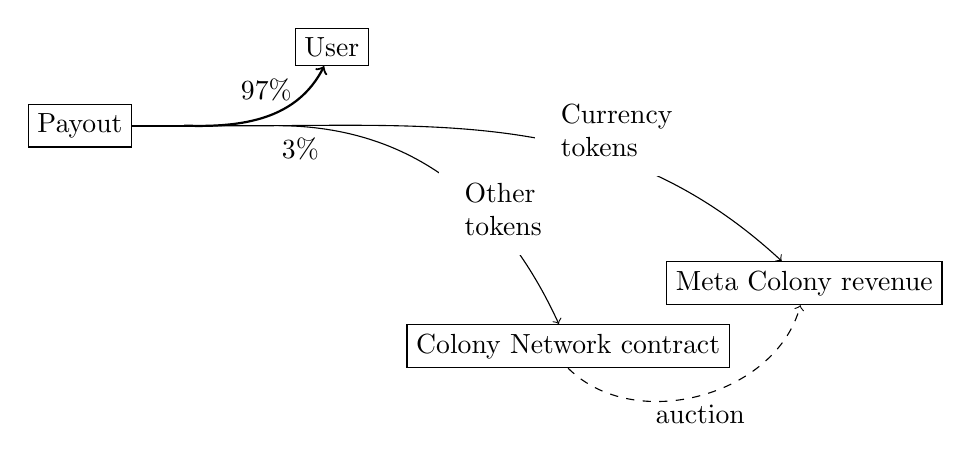
\begin{tikzpicture}
  \node at (-4,0) (dummy) {};
  \node[draw] at (-5.2,0) (bountybox) {Payout};
  \node at (-2.8,0) (bounty) {}
   (bountybox.east) edge[-, thick] (dummy.east)
   (dummy.east) edge[-] (bounty.east);
   \node at (-2.4,-0.3) {{3\%}};
  \node[draw] at (-2,1) (user) {User};
  \node[draw] at (1,-2.8) (cnc) {Colony Network contract};
  \node[draw] at (4,-2) (root) {\rc\ revenue}
    (dummy.east) edge[->, bend right=40,out=-25,thick] node[above=2pt] {97{\%}} (user)
    (dummy.east) edge[->, bend left=30,out=12] node[fill=white,right=10pt] {\begin{tabular}{l} Currency \\ tokens\end{tabular}} (root)
    (bounty.east) edge[->, bend left=30,out=35] node[fill=white, below right=-5pt] {\begin{tabular}{l} Other \\ tokens\end{tabular}} (cnc)
    (cnc.south) edge[->, bend right=60, dashed] node[below] {auction} (root)
    ;
 \end{tikzpicture}
 \caption{Summary of the revenue split upon payout for a task.}
 \label{fig:revenueSplit}

\end{figure}

This idea of a fee is a little unusual for such a decentralised system. One of the appeals of decentralised systems on Ethereum is that other than gas costs, they do not seek rent and are free to use. However, the network fee is key to ensuring the game theoretic security of the Colony Network's reputation mining and governance processes, by providing underlying value to the CLNY held by \rc\ members. Importantly, this fee is not payable to any centrally controlled entity, but rather to the \rc. As anybody may contribute to the \rc, anyone may claim a share of these fees proportional to their contribution. We believe that the benefit of being part of a secure, well maintained network will be appealing enough that a small fee to pay for its existence will be acceptable.

The presence of this fee means we have to make some considerations which would otherwise be irrelevant. Primarily, we will need to make `piggyback' contracts as hard as possible to make that might e.g. be used to pay out an expenditure payout when a expenditure was finalized, but without sending the fee.

\subsubsection{The token auction}

As the network fee may be denominated in any ERC20 token, there is a need for a mechanism to liquidate arbitrary bundles of tokens: the token auction. The tokens collected are auctioned off by the Colony Network Contract, with the auctions denominated in \rcts, the proceeds of which are burnt. These auctions --- one for each type of token collected --- occur on a regular basis of once a month.

We believe such a mechanism will be beneficial for the \rcths\ (whose tokens gain value by having an explicit use beyond reputation mining) and the \rc\ itself (by reducing the supply of \rcts\ and thus making any future minting more valuable). It also provides an immediate mechanism of price discovery for a colony's internal tokens, which are unlikely to be traded on third-party exchanges until much later in the lifetime of the colony. By auctioning off the collected tokens, we also prevent the \rc\ collecting a large number of different tokens that it has to manage, which would prove cumbersome and annoying.

\subsection{The \rc\ and CLNY}\label{sec:clny}

The \rc\ is a special colony which governs the Colony Network. Tokens in the \rc\ are known as CLNY and will be initially generated during the Colony Network distribution period.\footnote{The mechanism of this distribution are yet to be defined.}

\subsubsection{Role of CLNY holders and the \rc}

CLNY holders have two primary roles. The first is to participate in the reputation mining process, described in Section \ref{sec:reputationmining}. The second is management of the Colony Network itself. There will be permissioned functions on the Network Contract to allow fundamental parameters of the network to be set, which can only be called by the \rc. For these permissioned functions to be called by the \rc, a vote open to all CLNY and reputation holders must be conducted.

Management of the Colony Network also includes making updates to Colony contracts available to colonies. CLNY holders are not necessarily responsible for the development of these updates, but are required to vote to deploy them. They are therefore responsible for at least ensuring due diligence is done, either by themselves or by service providers, to avoid introducing security weaknesses or other undesirable behaviour. In return for the responsibility of the development and maintenance of the Colony Network, the \rc\ is the beneficiary of the network fee (see Section \ref{sec:networkrevenue}).

Reputation in the \rc\ can be acquired by earning CLNY tokens via expenditure payouts just as in any other colony (see Section \ref{sec:earning-losing-rep}). Reputation in the \rc\ can also be earned by participating in the reputation mining process (see Section \ref{subsec:mining-costs-and-rewards}), which is unique to the \rc.

\subsubsection{Handing off decision-making power to the \rc}\label{subsec:ceding-control-to-rc}

\rct\ holders are responsible for reputation mining from the start, but decisions about the underlying properties of the network will initially be made by a multisignature contract controlled by the Colony team. As the network develops and is proved to be effective, control over these decisions will cede to the \rc.

\subsubsection*{Stage 1: Colony team multisig in control}
 Initially, the Network Contract's functions will be \textbf{root}-permissioned to only allow transactions from the multisig contract under the control of the Colony team to change these properties of the network.

\subsubsection*{Stage 2: Colony team multisig approval required}
At a later date, an extension contract will be set up and given the \textbf{root} permission. This contract will allow the \rc\ (as a whole, via the governance mechanisms provided to all colonies) to propose changes to be made to the Colony Network Contract. The intermediate contract will have functionality such that all changes will have to be explicitly allowed by the account under the control of the Colony team. In other words, the \rc\ will be able to propose changes, but the team must sign them off.

\subsubsection*{Stage 3: Colony team multisig retains veto}
The next stage will be a second extension contract operating similarly to the first, but after a timeout --- with no interaction from the Colony team's account --- the change will be able to be forwarded to the Colony Network Contract by anyone. The Colony team's role will be to block changes if necessary. Thus at this stage the \rc\ will be able to make changes autonomously, but the Colony team retains a veto.  The proposal to move to this contract will have to come from the \rc\ itself.

\subsubsection*{Stage 4: \rc\ fully controls the network}
Finally, the specialized extension contract will be removed and replaced with a generic voting extension (see Section \ref{sec:motions-and-disputes}), and the \rc\ will have direct control over the Colony Network Contract with no privileged control available to the Colony team other than that provided by any CLNY and reputation held.

\newpage
\section{CLNY Tokens and the Meta Colony}\label{sec:clny}

\subsection{Creation of CLNY tokens}
After the Colony Network Contract is deployed, the first colony created will be the \rc. Tokens in the Meta Colony will be known as CLNY. CLNY will be initially generated during the Colony Network distribution period.\footnote{The mechanism of this distribution are yet to be defined.}

Functionality will be added to the CLNY token contract as required, through the \code{EtherRouter} mechanism described in Section  \ref{subsec:upgradability}. The ability to add functionality is extremely powerful, and theoretically could allow the inclusion of additional functions to arbitrarily set balances or create additional tokens. This would destroy trust in CLNY, and thereby its underlying utility. For this reason, the ability to add new functionality to the CLNY token will never lie with the developers of Colony, but with a multisignature contract initially made up of members of the wider Ethereum community, and then subsequently the \rc\ itself.

\subsection{Role of CLNY holders and the \rc}
CLNY holders have two primary roles. The first is to participate in the \textbf{Reputation Mining} process, described in Section \ref{sec:reputationmining}.

The second is management of the Colony Network itself. There will be permissioned functions on the Network Contract to allow fundamental parameters of the network to be set, which can only be called by the \rc.

For these permissioned functions to be called by the \rc, a vote open to all CLNY and reputation holders must be conducted  (see Section \ref{sec:arbitrary-transaction}).

Management of the Colony Network also includes making updates to Colony contracts available to colonies. CLNY holders are not necessarily responsible for the development of these updates, but are required to vote to deploy them. They are therefore responsible for at least ensuring due diligence is done, either by themselves or by service providers, to avoid introducing security weaknesses or other undesirable behaviour.

In return for the responsibility of the development and maintenance of the Colony Network, the \rc\ is the beneficiary of the network fee (see Section \ref{sec:networkrevenue}).

Reputation in the \rc\ can be acquired by earning CLNY tokens completing tasks, and administrative and evaluative duties just as in any other colony (see Section \ref{sec:earning-losing-rep}). Reputation in the \rc\ can also be earned by participating in the reputation mining process (defined in Section \ref{subsec:mining-costs-and-rewards}), which is unique to the \rc.

\subsection{Handing off decision-making power to the \rc}\label{subsec:ceding-control-to-rc}
\rct\ holders are responsible for Reputation Mining from the start, but decisions about the underlying properties of the network will initially be made by a multisignature contract controlled by the Colony team. As the network develops and is proved to be effective, control over these decisions will cede to the \rc.

\subsubsection*{Stage 1: Colony team multisig in control}
 Initially, the Network Contract's functions will be permissioned to only allow transactions from the multisig address under the control of the Colony team to change these properties of the network.

\subsubsection*{Stage 2: Colony team multisig approval required}
At a later date, an intermediate contract will be set up, to receive these permissions. This contract will allow the \rc\ (as a whole, via the governance mechanisms provided to all colonies) to propose changes to be made to the Colony Network Contract. The intermediate contract will have functionality such that all changes will have to be explicitly allowed by the address under the control of the Colony team. In other words, the \rc\ will be able to propose changes, but the team must sign them off.

\subsubsection*{Stage 3: Colony team multisig retains veto}
The next stage will be a second intermediate contract operating similarly to the first, but after a timeout --- with no interaction from the Colony team's address --- the change will be able to be forwarded to the Colony Network Contract by anyone. The Colony team's role will be to block changes if necessary. Thus at this stage the \rc\ will be able to make changes autonomously, but the Colony team retains a veto.  The proposal to move to this contract will have to come from the \rc\ itself.

\subsubsection*{Stage 4: \rc\ fully controls the network}
Finally, the intermediate contract will be removed, and the \rc\ will have direct control over the Colony Network Contract with no privileged control available to the Colony team other than that provided by any CLNY and reputation held.


\newpage
\section{Structure of a Colony}\label{sec:colony-structure}
Colonies exist to enable collaboration between their members, and direct collective efforts towards common goals. Facilitating effective division of labour, management of incentives, and allocation of resources are therefore some of the most important functions of the Colony protocol.

\subsection{Domains and permissions}\label{sec:domains}\label{sec:permissions}

The essential structure of the colony revolves around domains and the permissions that accounts may have in them. These two concepts jointly define the structure and security of a colony and provide a flexible framework for creating colonies of many kinds.

\subsubsection{Domains}

Like any organization, without structure, a large colony would quickly become difficult to navigate due to the sheer number of participants and interactions taking place --- domains solve this problem. A domain is like a folder in a shared filesystem, except instead of containing files and folders, it can contain subdomains, funding, and expenditures. This simple modularity enables great flexibility as to how an organisation may be structured. Domains could be used to represent teams, departments, projects, tribes, circles, and so forth. A toy example is shown in in Figure \ref{fig:domainhierarchysample}.

\begin{figure}[h]
    \centering
 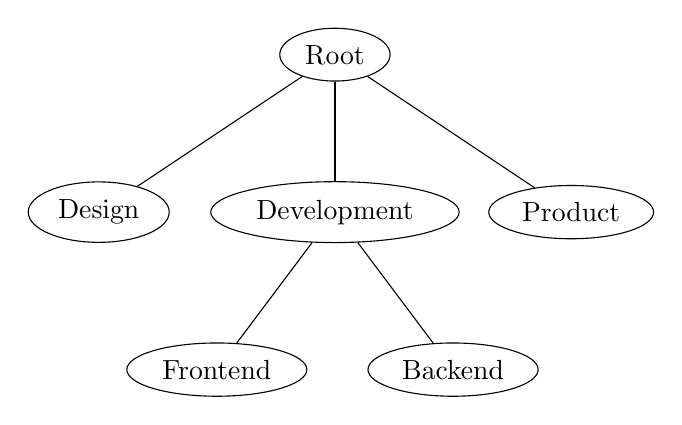
\begin{tikzpicture}
   \node[shape=ellipse, draw] at (0,0) (tld) {Root};

   \node[shape=ellipse, draw] at (-3,-2) (design) {Design}
    (tld) edge[-] (design);

   \node[shape=ellipse, draw] at (0,-2) (development) {Development}
    (tld) edge[-] (development);

   \node[shape=ellipse, draw] at (3,-2) (product) {Product}
    (tld) edge[-] (product);

   \node[shape=ellipse, draw] at (-1.5,-4) (frontend) {Frontend}
    (development) edge[-] (frontend);

   \node[shape=ellipse, draw] at (1.5,-4) (backend) {Backend}
    (development)  edge[-] (backend);
 \end{tikzpicture}
 \caption{Parts of a domain hierarchy for a colony developing a web service.}
 \label{fig:domainhierarchysample}
\end{figure}

It is ultimately up to individual colonies to decide how they wish to use domains—some might only use them for coarse categorisations, whereas others may use them to precisely group only the most similar expenditures together, or even multiple expenditures that other colonies would consider a single expenditure. Some might use domains to represent long-lived organizational departments, while others might use them more ephemerally, to represent projects with start and end dates. We aim to provide a general framework that colonies may use however they see fit, and to be prescriptive only where necessary.

Among other things, this compartmentalisation of activity provides an essential benefit to the colony as a whole by making reputation \textit{contextual}. When arbitration occurs, it occurs at a specific level in the colony's domain hierarchy. This means that people with relevant contextual knowledge can be included for their opinion, and that when arbitration occurs, the whole colony is not required to participate in the process.

\subsubsection{Permissions}

Access control in a colony is organized around the concepts of \textbf{permissions}. There are six different permissions (roughly in order of influence): recovery, root, arbitration, architecture, funding, and administration, each unlocking a bundle of semantically-related functionality.

With the exception of the recovery and root permissions, all permissions are domain-specific (much like permissions in a Unix file system are directory-specific), with the rule that permissions held in a parent domain are inherited in all child domains. Put another way, have a permission in a domain gives you that permission in the entire \textit{subtree} rooted in that domain. To implement this inheritance, permissioned functions require a \textit{domain proof} of the following arguments:

\begin{itemize}
\item \texttt{permissionDomainId} - The (parent) domain in which the account holds the permission.
\item \texttt{childSkillIndex} - The index of \texttt{domainId} in \texttt{permissionDomainId}'s \texttt{children} array.
\item \texttt{domainId} - The (child) domain in which the action is being taken.
\end{itemize}

These arguments can be evaluated on-chain in constant time to determine whether the account is authorized to call the privileged function.

Permissions are held by Ethereum accounts. This means that permissions may be given to human administrators, or assigned to contracts which implement more complex behavior (such as voting mechanisms). These types of contracts are known as \textbf{extensions} and are discussed in-depth in Section \ref{sec:extensions}. The use of extensions to flexibly `plug-in' various decision-making mechanisms is a key concept in the Colony protocol.

It is worth noting that the list of accounts that have the permission in question have the full permission; no additional restrictions exist at the protocol level. In some cases, these are extremely powerful capabilities (such as emitting arbitrary reputation penalties) and require absolute confidence in whomever or whatever controls it. We anticipate therefore that in many cases, extension contracts will be used to offer varying degree of moderation to the underlying permissions.

\subsubsection*{Recovery}

The recovery permission gives accounts access to the colony's emergency `recovery' functionality, which allows for arbitrary state-changes to the colony's data. Recovery mode is described in more detail in Section \ref{sec:escape-hatches}.

\subsubsection*{Root}

The root permission gives accounts access to high-level administrative functions in the colony, such as setting colony-wide parameters, upgrading the colony, and minting new internal tokens. This permission also gives accounts the ability to assign permissions throughout the colony (including in the root domain).

\subsubsection*{Arbitration}

The arbitration permission gives accounts the ability to make domain-specific state changes, meant as a means of resolving motions. This permission also enables accounts to emit reputation penalties (but not reputation increases).

\subsubsection*{Architecture}

The architecture permission gives accounts the ability to create new domains in a colony, as well as assign permissions in those new domains. Unlike root, accounts with this permission cannot edit permissions in the domain in which they hold the permission, only in subdomains.

\subsubsection*{Funding}

The funding permission gives accounts the ability to move tokens between funding pots. In practice, this means that this permission is responsible for allocating money amongst domains and for funding expenditures. Financial management in a colony is described in more detail in Section \ref{sec:finance}.

\subsubsection*{Administration}

The administration permission gives accounts the ability to create and manage (but not fund) expenditures, the basic incentive unit in a colony, described in Section \ref{sec:expenditures}. \\

Broadly, permissions are designed as a `separation of powers': different permissions must work in concert to carry out the functioning of a colony. For example, administration can create an expenditure, but only funding can actually provide the resources, while arbitration resolves motions as they arise. Complex extensions may require multiple permissions in order to function properly (such as `tasks', which requires both arbitration and administration).

The intention is that, since permissions are grouped into semantic bundles of functionality, it will be possible to develop \textit{specialized} mechanisms for mediating access to the underlying functionality (i.e. specialized funding mechanisms and specialized dispute-resolution mechanisms, as opposed to a general-purpose `voting' mechanism meant to handle all possible decisions).

Colony's long-term vision is of \textit{trustless organizations}; organizations in which members can safely collaborate and manage shared resources, without needing to know or trust each other. Early colonies may find that a larger emphasis on human moderators to be useful, while more mature colonies may find reasons to devolve increasingly more decision-making to extensions implementing trustless functionality. We will refer to colonies which make substantial use of these extensions as \textit{trustless colonies}.

\subsection{Funding and expenditures}\label{sec:expenditures}\label{sec:finance}

All tokens and currencies are administered by the colony contract; it is responsible for all the bookkeeping and allocations. The former are managed via funding pots, the latter via expenditures.

\subsubsection{Funding pots}

Each domain and each expenditure in a colony has an associated \emph{funding pot}. A funding pot can be thought of as a wallet specific to a particular domain or expenditure, and are used to move funds around \textit{within} a colony. To each funding pot, the colony contract may associate any number of Ether or ERC20-compatible tokens it holds. Depending on context, the funds in a funding pot may be referred to as the payout, bounty, budget, salary or working capital. In addition to the funding pots, there is a special \emph{rewards pot} which accumulates tokens to be distributed to members as \textit{rewards} (see Section \ref{sec:revenue}).

Only accounts holding the \textbf{funding} permission may move tokens; the rule is that they may move tokens between any two pots in the subtree rooted in the domain in which they hold the permission. It is the expectation that this permission will in many cases be given to an \textit{extension contract} implementing a specialized decision-making mechanism, such as the \textit{funding queue} described in Section \ref{sec:funding-queues}.

\subsubsection{Expenditures}

The basic payment primitive of a colony is the `expenditure'. Expenditures are used to transfer funds out of a colony to any Ethereum account. An expenditure has several properties:

\begin{itemize}
\item An \texttt{owner} (the account address which created the expenditure).
\item A \texttt{status} (active, cancelled, or finalized).
\item One or more \texttt{recipient}s.
\item \texttt{payouts} for each recipient, denominated in one or more tokens.
\item Optionally, a per-recipient \texttt{skill}.
\item Optionally, a per-recipient \texttt{payoutModifier}.
\item Optionally, a per-recipient \texttt{claimDelay}.
\end{itemize}

The owner is responsible for setting the properties of the expenditure. The recipients are simply Ethereum accounts. While it is anticipated that recipients will be individuals, there is nothing to prevent these accounts being contracts under the control of multiple people.\footnote{With the protocol as described in this document, any reputation earned would be assigned to the contract in question and not able to be moved to the appropriate users. In these cases, it might be better to develop an extension contract which would determine the per-user allocation in advance and configure the expenditure accordingly.}

Once the expenditure is finalized, all properties become locked (but subject to arbitration) and payouts can be claimed (and reputation awarded). Prior to finalization, the owner has the ability to cancel the expenditure entirely. Any funds that have already been assigned to the expenditure can be reassigned to the domain that the expenditure was created in.

Defining the payouts for each recipient, of course, does not provide the funds --- this must be done through the funding mechanisms in Colony. Payouts do not have to all be in the same token, and an expenditure's payouts can be made up of an arbitrary number of tokens.

The expenditure is meant to be an abstract primitive which can support many types of workflows, and so contains optional attributes to support more complex behavior (see Section \ref{sec:extensions}). For instance, the \texttt{payoutModifier} and \texttt{claimDelay} can be used to implement a rating and review system, where good or bad reviews lead to an across-the-board reputation increase (or payout decrease) for a recipient, while the \texttt{claimDelay} is set to allow for any relevant motions to be decided before funds can exit the colony. \\

Once the tokens have been received by an account, they are under the control of the recipient --- there is no way to reclaim the funds. The funds have to cross the `Cryptographic Rubicon' somewhere in the system (by the nature of the blockchain), and it makes sense to do so here.\footnote{Currently, the only way this rule can be broken is by the Colony conspiring to abuse the `arbitrary transaction' feature described in Section \ref{sec:arbitrary-transaction}.}

\subsection{Internal tokens}\label{sec:colony-tokens}

Every colony has its own ERC20-compatible `internal token'. These are the tokens that, when earned as an expenditure payout, also generate reputation for the receiver (and thus distribute control within the colony). What these tokens represent apart from this is up to the colony to decide. For example, they may have financial value, or they may be purely symbolic; some possible scenarios are outlined in this section.

In addition, colonies may `bring their own token' and designate an existing ERC20-compatible token as reputation-bearing. While this may be advantageous in some contexts, it’s worth noting that this weakens the incentive alignment underpinning the game theoretic security of trustless colonies, in that the value of the token is divorced from the performance of the colony. Note that the internal token cannot be changed once a colony has been created, so \textit{choose wisely}.

In cases where a colony creates a new token, that colony is in control of the supply of the token. Specifically, \textbf{root} permission holders can mint tokens at-will. In some cases, this may look like a founder managing the token supply unilaterally, while in other cases colonies may manage the minting process via an extension contract (see Section \ref{sec:colony-token-management} for an example).

A common question is why only internal tokens (as opposed to all tokens) are reputation-bearing. The reason for having a single token be reputation-bearing is that it avoids tricky exchange-rate problems, such as incentives to receive more of a less valuable token to earn more reputation.

\subsubsection{Token use-cases}

Ultimately, internal tokens are used to distribute reputation, and thus both ownership and decision-making power. Since users with more reputation can both exercise more influence over the activity of the colony, as well as claim a greater share of the rewards, reputation functions to align incentives among the members of colony. Here we give a few examples of different use-cases for internal tokens, demonstrating the variety of schemes colonies may adopt for distributing ownership and influence alongside cash compensation.

\subsubsection*{Tokens as early rewards}

One of the chief benefits of a colony having its own token is that it can offer rewards for work before it has any revenue or external funding to draw on. A new colony may offer token payouts for expenditures with the hope that the reputation earned by these token payments (and the future revenue earned by the colony) will eventually lead to financial rewards. By allowing `spending' before fund-raising, the financial burden during the start-up phase of a new colony is eased. Once a colony is profitable, payment in tokens may be the exception rather than the norm.

\subsubsection*{Tokens representing hours worked}

We could imagine a colony in which all expenditures are paid in Ether, but include a number of the colony's own tokens as well, equal to the expected number of hours worked. The members of the colony would be responsible for assigning `correct' token and Ether payouts to expenditures. This extra responsibility would also ensure users doing the same amount of work received the same reputation gain, rather than the reputation gain being dependent on the rates they charged.

\subsubsection*{Tokens as performance-based bonuses}

Alternatively, we could imagine a colony which seeks to balance predictable compensation (i.e. salaries) with performance-based incentives. Such a colony could pay out salaries in a token such as Ether or DAI, and reserve their internal token for performance-based bonuses (i.e. for hitting quarterly OKRs). Such an approach makes reputation (and decision-making power) a function of achievement, without making members of the colony feel as though their ability to pay rent depends on their ability to hit quarterly goals.

\subsubsection{Colony's \ascode{Token} contract}

Colony has developed a customized \ascode{Token} contract, with some additional functionality:

\begin{itemize}
	\item \ascode{mint} --- lets the token contract owner introduce new tokens into circulation.
	\item \ascode{burn} --- lets anyone permanently remove tokens from circulation.
\end{itemize}

In addition, Colony's \ascode{Token} contract introduces the idea of `locking' --- tokens being non-transferrable until a one-way boolean flag is flipped. This is useful for colonies which want more control over how and when their tokens can be liquidated and exchanged.

This contract underlies the \rct\ (see Section \ref{sec:clny}) and is the default token contract for new colonies, although colonies are free to choose any ERC20-compatible token.

\subsection{Revenue and rewards}\label{sec:revenue}

A colony may sell goods and services in exchange for Ether or any ERC20-compatible tokens, and this revenue may be sent to the colony's address. Whenever a colony receives such payments, we say that the colony has earned \emph{revenue}. Revenue is distinct from a colony's working capital: the latter is the sum of all tokens held by the colony in various domains (see Section \ref{sec:finance}), while the former is implicitly defined as the colony's token holdings not yet accounted for in any of the existing pots.

There is an expectation that some fraction of any Ether or other tokens received by the colony are paid out to their members. `Members', in this context, means accounts holding both tokens and reputation in the colony. Whenever a colony distributes a portion of revenue to its members, we say that the colony is paying out \emph{rewards}.

\subsubsection{Processing revenue}

Revenue accumulates as the colony receives transfers of tokens. In order to be processed, any user can make a special \texttt{claimColonyFunds} transaction, indicating for which token they wish to process accumulated revenue.

The transaction then calculates the amount of token-denominated revenue that has accumulated since the last such transaction, and transfers some proportion to the colony's rewards pot. The remainder is then made available to the colony as working capital. The percentage split is configurable by the \textbf{root} permission via the \texttt{setRewardInverse} function.

\subsubsection{Claiming rewards from the rewards pot}\label{sec:claimrewards}

Rewards accumulate in the rewards pot. To trigger a payout to users (i.e. to make rewards claimable) a \textbf{root} user makes a special \texttt{startNextRewardPayout} transaction (no more than once every \rewardclaimduration\ days), initiating a process by which all members may claim a payout based on the reward pot's holdings.

This reward payout transaction includes the specific currency that should be paid (reward payouts for each token are handled separately). Once the process begins, all users' tokens are locked until they claim their payout. Locking is necessary because the token balance of each account factors into the rewards formula of equation \eqref{eq:reward-claim}. Locking is done by incrementing the token's \texttt{totalLockCount}.

Our \texttt{TokenLocking} contract contains a locking mechanism ensuring that a user cannot move tokens while they have (token-weighted) votes to reveal; we use the same mechanism here to ensure that a user cannot move tokens after a payout is approved by the members of the colony but before the user has claimed their rewards. The colony has a counter for each user that is incremented whenever they claim a payout; they can also waive their claim to a payout that will increment this counter. \\

\textbf{Rewards are only available to accounts that hold both tokens and reputation}, and the amount claimable by each account depends on \emph{both} token balance and reputation (see equation \eqref{eq:reward-claim} below). Therefore we need to have a similar behaviour to `lock' the reputation of the users for the payout. When a payout is activated, the current state of the reputation tree is recorded in the payout itself. Users are paid out according to their reputation in this state, rather than the most recent state, to ensure all users get an appropriate payout and to avoid exploiting the system (which might otherwise be possible via e.g. delaying reward collection until after completing an expenditure, increasing their reputation).

\subsubsection{The rewards formula}

The amount that each user ($u_i$) of a colony ($\mathcal{C}$) is entitled to claim ($p_i$) is a function of their colony token holdings ($t_i$) and their total reputation in the colony ($r_i$):

\begin{equation}\label{eq:reward-claim}
 p_i = \left(\frac{t_i r_i}{T \times R}\right)^{\frac{1}{2}} \qquad \textnormal{where} \quad T = \sum\limits_{u_j\in \mathcal{C}} t_j \quad\textnormal{and}\quad R = \sum\limits_{u_j\in \mathcal{C}} r_j.
\end{equation}

This is a (normalised) geometric average of the user's token holdings and reputation. We note that this is very unlikely to payout all the tokens set aside for a payout --- the only way it would do so is if everyone had the same proportion of reputation in the colony as they did proportion of tokens in the colony. However, the geometric average is the natural way to fairly capture the influence of two variables with different ranges, and ensures that large token holders must earn large amounts of reputation to get the most from the payouts. The total reputation and user reputation in the colony are all provable on-chain at claim time via a Merkle proof that the \ascode{ReputationRootHash} (Section \ref{sec:reputationmining}) contains some values claimed by the user; the user's balance of colony tokens and the total number of tokens issued is trivial to lookup.

After some sufficiently long period of time (\rewardclaimduration\ days), all unclaimed tokens can be reclaimed on behalf of the colony by a user, and the payout closed. Any users that have not claimed their payout by that point will still have their tokens locked, and they will remain locked until they issue a transaction waiving their claim to the payout (indeed, they already passively did this by not claiming it in a timely fashion). Unclaimed tokens are returned to the rewards pot and become part of the next reward cycle.

\subsection{The reputation system}\label{sec:reputation}

Reputation is a number associated with each user which attempts to capture the value of that user's contributions to the colony over time. Reputation is used to weight a user's influence in decisions related to the expertise they have demonstrated, and to determine amounts owed to a colony's members when rewards are disbursed. Because reputation is awarded to users by either direct or indirect peer assessment of their actions, we argue that influence and rewards can be seen as being (roughly) distributed by merit. Colony's aim is that the reputation system will enable an emergent and dynamic decision-making hierarchy in which all of the right people are in the right places.

Colony aims to be broadly meritocratic. Consequently, the majority of decisions in a trustless colony are weighted by the relevant reputation. Unlike tokens, reputation cannot be transferred between accounts, as it represents an appraisal of the account's activities by their peers. Reputation must therefore be earned by direct action within the colony. Reputation that is earned will eventually be lost through inactivity, error, or misbehaviour; a description of how reputation is gained and lost is given in Section \ref{sec:earning-losing-rep}.

\subsubsection{Types of reputation}

\subsubsection*{Reputation by domain}\label{sec:rep-by-domain}

The hierarchical domain structure of a colony was described in Section \ref{sec:domains}. Reputation is earned in this hierarchy, and a user has a reputation in all domains that exist --- even if that reputation is zero. When a user earns or loses reputation in a domain, the reputation in all parent domains changes by the same amount. In the case of a user losing reputation, they also lose reputation in all child domains, but in this case the child domains lose the same \textit{fraction} of reputation that was lost in the original domain. If a reputation update would result in a user's reputation being less than zero, their reputation is set to zero instead. \\

\begin{figure}[h]
    \centering
 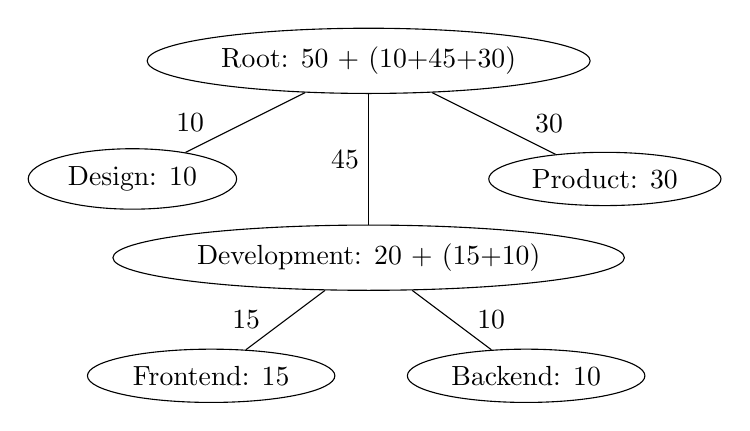
\begin{tikzpicture}
   \node[shape=ellipse, draw] at (0,0) (tld) {Root: 50 + (10+45+30)};

   \node[shape=ellipse, draw] at (-3,-1.5) (design) {Design: 10}
    (tld) edge[-] node[left=4mm] {10} (design);

   \node[shape=ellipse, draw] at (0,-2.5) (development) {Development: 20 + (15+10)}
    (tld) edge[-] node[left] {45}  (development);

   \node[shape=ellipse, draw] at (3,-1.5) (product) {Product: 30}
    (tld) edge[-] node[right=4mm] {30}  (product);

   \node[shape=ellipse, draw] at (-2,-4) (frontend) {Frontend: 15}
    (development) edge[-] node[left=2mm] {15}  (frontend);

   \node[shape=ellipse, draw] at (2,-4) (backend) {Backend: 10}
    (development)  edge[-] node[right=2mm] {10}  (backend);
 \end{tikzpicture}
 \caption{Reputation flowing up a domain hierarchy.}
 \label{fig:reputationhierarchysample}
\end{figure}

An example makes this clearer. Suppose a colony has a `development' domain which contains a `backend' domain and a `frontend' domain, as in Figure \ref{fig:reputationhierarchysample}. Any time a member of the colony earns reputation for work completed in the backend domain, it will increase their backend reputation, their development reputation and their reputation in the all-encompassing root domain of the colony. Reputation earned in the development domain will only increase the development and root domain reputation scores of the user.

Later, the user behaves badly in the `development' domain, and they lose 100 reputation out of the 2000 they have in that domain. They also lose 100 reputation in the parent domains, and 5\% $\left(\frac{100}{2000}\right)$ of their reputation in each of the child domains of the `development' domain (which in this example, includes both frontend and backend domains).

\subsubsection*{Reputation by skill}\label{sec:rep-by-skill}

We anticipate domains to mostly be used as an organisational hierarchy within a colony. However, this would not necessarily capture the \emph{type} of work that a user completed to earn their reputation. If the domain were a project, with expenditures involving both design and development work, reputation earned by completing expenditures related to these skills would not be distinguishable. To have a more granular account of the work a user completes to earn their reputation, a skill cloud is also maintained.

This global cloud of skill tags is available to all colonies, and is curated and maintained by the \rc. When an expenditure is created, as well as being placed in a particular domain in the colony, may also be tagged with one or more skills from the skills cloud. When the recipient earns reputation by claiming the payout, they will earn reputation in all skills the expenditure was tagged with, with the reputation divided uniformly amongst the skills. This is in addition to the reputation earned in the relevant domains.

Even though the skills cloud is universal, specific skills reputation is unique to each colony. Earning reputation in a skill in one colony has no effect on the user's reputation in that skill in any other colonies.

\subsubsection*{Reputation by colony}\label{sec:rep-by-colony}

A user's total reputation in a colony is their reputation in the root domain. This is the reputation they will be voting with in any decisions that require input from everyone in a trustless colony (i.e. modifying colony-wide parameters). Reputation in a colony has no effect outside the colony. In particular, reputations held in one colony have no bearing on reputations held by the same account in another colony.

\subsubsection{Earning and losing reputation}\label{sec:earning-losing-rep}

There are three ways to receive reputation in a colony.\footnote{The \rc\ is a special case where reputation may also be earned by reputation mining (see Section \ref{sec:reputationmining}).} The first (and by far the most common) is through receiving a payout via an expenditure. The second is through the arbitration process. The third is upon the creation of a colony and the associated bootstrapping process.

Reputation losses broadly occur as the result of arbitration, and extension contracts (see Section \ref{sec:extensions}) makes it possible to implement mechanisms which involve reputation penalties (such as tasks and disputes). In addition, all reputation earned by users is subject to a continual decay over time.

The rest of this section outlines each of these mechanisms, with references to the more detailed descriptions given elsewhere where appropriate.

\subsubsection*{Reputation change via expenditures}

Whenever an expenditure recipient receives a payout denominated in the colony's internal token, the recipient also receives some amount of reputation, scaled by that recipient's \texttt{payoutScalar}. A value of 1 gives reputation equivalent to the token payout, but a multiple of up to 2x is possible. The reputation is earned in the domain (and all parent domains) of the expenditure, and divided equally among any skills associated with that recipient.

\subsubsection*{Reputation change as a result of arbitration}\label{sec:earning-rep-in-disputes}

Arbitration permission holders have the ability to emit arbitrary reputation penalties (but not increases) in both domains and skills. While this might seem to be a significant power available to arbitration permission holders, recall that this permission will in many cases be assigned to extension contracts, which will mediate this ability via various mechanisms, such as the motions system (see Section \ref{sec:motions-and-disputes}).

\subsubsection*{Bootstrapping reputation}\label{sec:bootstrapping-rep}

Since a trustless colony's decision making procedure rests on reputation weighted voting, we are presented with a bootstrapping problem for new colonies. When a trustless colony is new, no-one has yet completed any work in it and so nobody will have earned any reputation. Consequently, no motions can be made and no disputes can be resolved as no-one is able to vote. Then, once the first expenditure is paid out, that user has a dictatorship over decisions in the same domains or skills until another user earns similar types of reputation.

To prevent this, when a colony is created, the creator can choose accounts to have initial reputation assigned to them in the root domain to allow the colony to bootstrap itself. The reputation assigned to each user will be equal to the number of tokens received, i.e. if a member receives ten tokens, they also receive ten reputation in the root domain. Given that reputation decays over time, this initial bootstrapping will not have an impact on the long-term operation of the colony. This is the only time that reputation can be created without an associated expenditure being paid out. Users receiving reputation are presumably the colony founder and their colleagues, and this starting reputation should be seen as a representation of the existing trust which exists within the team.

We note that the same is not required when a new domain is created in a colony. We do not wish to allow the creation of new reputation here, as this would devalue reputation already earned elsewhere in the colony. This bootstrapping issue is resolved by instead using reputation within the parent domain, when a child domain contains less than 10\% of the reputation of its parent domain. A domain below this threshold cannot have domains created under it.

\subsubsection*{Reputation decay}

All reputation decays over time. Every \repdecayduration\ days,\footnote{It is likely that this parameter will be configurable on a per-colony basis in the future.} a user's reputation in every domain or skill decays by a factor of 2. This decay occurs every \miningcycleduration\ hour, rather than being a step change every \repdecayduration\ days to ensure there are minimal incentives to earn reputation at any particular time. This frequent, network-wide update is the primary reason for the existence of the reputation mining protocol, which allows this near-continuous decay to be calculated off-chain without gas limits, and then realised on-chain.

The decay serves multiple purposes. It ensures that reputation scores represent \emph{recent} contributions to a colony incentivising members to continually contribute to the colony. It further ensures that wild appreciations in token value (and the corresponding decrease in tokens paid per expenditure) do not permanently distort the distribution of reputation but instead serves to smooth out the effects of such fluctuations over time. \\

One might wonder why we have chosen to \textit{decay} reputation, rather than pursue a strategy of reputation \textit{dilution} via inflation. In one sense, they are equivalent: decaying reputation that is earned at a constant rate is the same as earning reputation at increasingly inflated valuations. Mathematically, however, decay is the cleaner approach, and so the use-case for inflation is that it is more feasibly calculated on-chain. In the case of Colony, reputation cannot be calculated on chain, since reputation updates effect an unbounded number of reputation nodes (due to the unbounded size of the domain tree). Since reputation cannot be calculated on chain, we choose to decay reputation in our off-chain reputation mining process.

\subsubsection{On-chain representation of skills and domains}\label{subsec:on-chain-representation-of-skills}

In the context of reputation, domains and skills are the same, differing only in that domains are colony-specific categorisation and skills are universal categorisation. In this subsection, each instance of `skill' should be taken to mean `skill or domain'.

Each skill that reputation can be earned in is assigned a \ascode{skillId} that is unique across the whole network. When a skill is created, additional properties are recorded and initialised.

\begin{equation*}
  \ascode{skillId} \rightarrow
  \begin{cases}
    \ascode{nParents} &	\textnormal{total number of parent skills.}\\
    \ascode{nChildren} &	\textnormal{total number of child skills.}\\
    \ascode{parents}\left[\cdots\right] &	\parbox[t]{.6\linewidth}{\textnormal{array of \ascode{skillId}s of a \textit{logarithmic subset} of parent skills, where \ascode{parents[i]} gives the $2^i$-th parent.}}\\
    \ascode{children}\left[\cdots\right] &	\textnormal{array of \ascode{skillId}s of \textit{all} child skills.}\\
    \ascode{globalSkill} &	\textnormal{whether the skill is a skill or domain.}\\
    \ascode{deprecated} &	\textnormal{whether the skill has been deprecated.}
  \end{cases}
\end{equation*}

Upon creation, \ascode{nChildren} is 0 and \ascode{children[]} is empty. These two attributes in all parents are updated with the \ascode{skillId} of the new child skill on creation.\footnote{We acknowledge that this is fundamentally gas limited, but the only consequence of this will be the inability to create new skills once the maximum depth allowed by the block size is reached. Our calculations suggest this corresponds to a depth of around 80, which we believe  is likely to be sufficient for the majority of use cases.}

Storing these pieces of data on-chain is required, as they are used by the reputation mining protocol (see Section \ref{sec:reputationmining}) and the procedures for appealing motions (see Section \ref{sec:motions-and-disputes}). They are stored under the control of the \ascode{ColonyNetwork} contract.

\subsubsection{Reputation update log}\label{subsec:reputation-update-log}

Whenever an event that causes one or more users to have their reputation updated in a colony occurs, a corresponding entry is recorded in a log in the \code{ColonyNetwork} contract. Each entry in the log contains:

\begin{itemize}
\item The user experiencing the reputation loss or gain.
\item The amount of reputation to be lost or gained.
\item The \texttt{skillId} of the reputation to be lost or gained.
\item The colony the update has occurred in.
\item How many reputation entries will need to be updated (including parent, child and colony-wide total reputations). This is the motivation for storing \ascode{nParents} and \ascode{nChildren} for each skill and domain.
\item How many total updates to reputations have occurred before this one in this cycle, including decays and updates to parents and children.
\end{itemize}

If the reputation update is the result of a dispute being resolved (as outlined in Section \ref{sec:earning-rep-in-disputes}), then instead of these first three properties, there is a reference to the dispute-specific record of stakes in the relevant colony. For the structure of this log, and an explanation of the way that it allows individual updates to be extracted in constant gas, see Appendix \ref{appendix:rep-transfer}.

This log exists to define an ordering of all reputation updates in a reputation update cycle that is accessible on-chain. In the event of a dispute during the reputation mining protocol (described in Section \ref{sec:reputationmining}), the \ascode{ColonyNetwork} contract can use this record to establish whether an update has been included correctly.

\subsection{Managing stakes}\label{sec:stakes}

Staking is a key concept in trustless systems, as a way to ensure that participants have `skin in the game' and can be incentivized towards good behavior. As Colony wishes to enable an ecosystem of extensions implementing various cryptoeconomic mechanisms (see Section \ref{sec:extensions}), a shared system for managing stakes improves usability and security by saving users from needing to send and retrieve tokens to and from many different contracts. In colonies, all stakes are denominated in that colony's internal token.

\subsubsection{Storing Tokens}

All stakes are stored in the network-wide \texttt{TokenLocking} contract. A singleton contract has the advantage that in scenarios where a user is a member of multiple colonies sharing the same internal token, a single deposit suffices for all colonies.

Any slashing of stakes occurs as a result of a function call coming from the \textit{colony} and is a result of colony-specific arbitration logic.

\subsubsection{Approvals and Obligations}

Stakes are managed via a sequence of \textit{approvals} and \textit{obligations}. Users \textit{approve} an account to then \textit{obligate} them up to the maximum amount of their approval. If an obligation is made in excess of the deposits held in the \texttt{TokenLocking} contract, the transaction will fail. Once an obligation is made, a user cannot withdraw tokens if the withdrawal would result in a balance less than their obligations. At any time, the approved extension can \textit{deobligate} the user, freeing the tokens for withdrawal (see Figure \ref{fig:stake-deobligate}). In practice, we expect that the same underlying deposit will be obligated and deobligated repeatedly without the user needing to move any additional tokens.

\begin{figure}[h]
    \centering
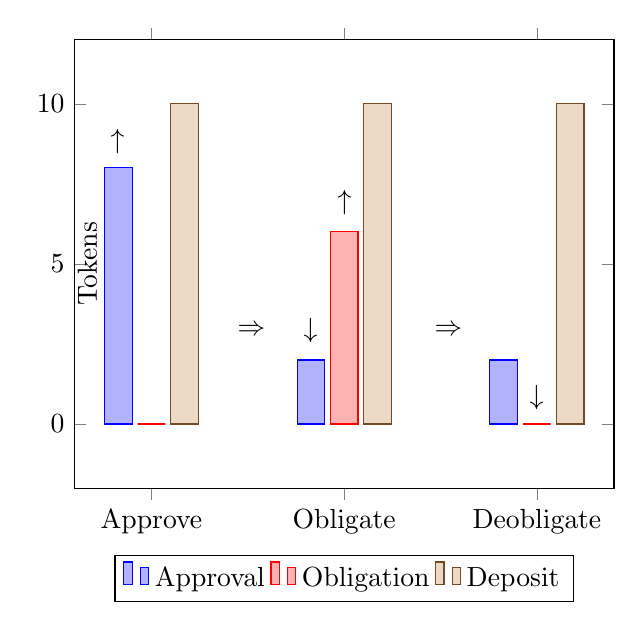
\begin{tikzpicture}
\begin{axis}[
    ybar,
    enlargelimits=0.2,
    legend style={at={(0.5,-0.15)},
      anchor=north,legend columns=-1},
    ylabel={Tokens},
    y label style={at={(axis description cs:.06,.5)}},
    symbolic x coords={Approve,Obligate,Deobligate},
    xtick=data,
    ]
\addplot coordinates {(Approve,8) (Obligate,2) (Deobligate,2)};
\addplot coordinates {(Approve,0) (Obligate,6) (Deobligate,0)};
\addplot coordinates {(Approve,10) (Obligate,10) (Deobligate,10)};
\legend{Approval,Obligation,Deposit}
\end{axis}
% Add the arrows
\node[] at (2.25,2) (x) {$\Rightarrow$};
\node[] at (4.75,2) (y) {$\Rightarrow$};
% Approve
\node[] at (.55,4.4) (x) {$\uparrow$};
% Obligate
\node[] at (3,2) (x) {$\downarrow$};
\node[] at (3.43,3.62) (x) {$\uparrow$};
% Deobligate
\node[] at (5.87,1.15) (x) {$\downarrow$};
\end{tikzpicture}
 \caption{Example stake lifecycle with deobligation}
 \label{fig:stake-deobligate}
\end{figure}

While an obligation is active, any \textbf{arbitration} permission holder can \textit{slash} the stake up to the amount of the obligation (see Figure \ref{fig:stake-slash}). We reiterate that this is a powerful ability and in most cases should be mediated by an appropriate extension (such as motions, described in Section \ref{sec:motions-and-disputes}).

\begin{figure}[h]
    \centering
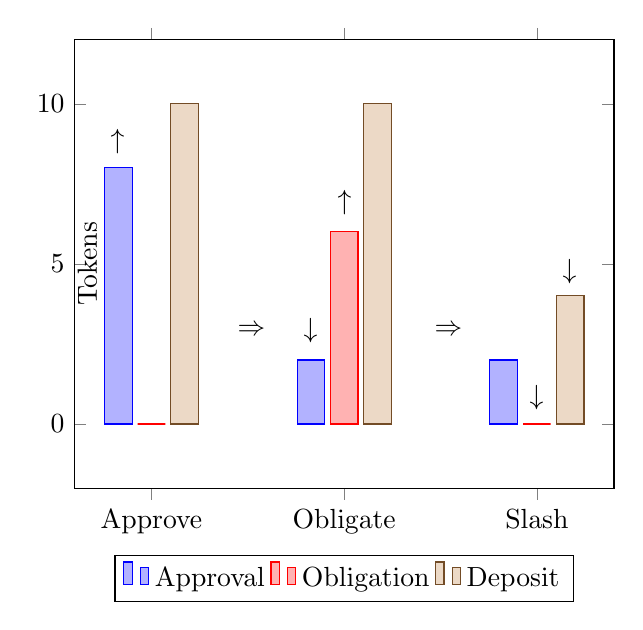
\begin{tikzpicture}
\begin{axis}[
    ybar,
    enlargelimits=0.2,
    legend style={at={(0.5,-0.15)},
      anchor=north,legend columns=-1},
    ylabel={Tokens},
    y label style={at={(axis description cs:.06,.5)}},
    symbolic x coords={Approve,Obligate,Slash},
    xtick=data,
    ]
\addplot coordinates {(Approve,8) (Obligate,2) (Slash,2)};
\addplot coordinates {(Approve,0) (Obligate,6) (Slash,0)};
\addplot coordinates {(Approve,10) (Obligate,10) (Slash,4)};
\legend{Approval,Obligation,Deposit}
\end{axis}
% Add the arrows
\node[] at (2.25,2) (x) {$\Rightarrow$};
\node[] at (4.75,2) (y) {$\Rightarrow$};
% Approve
\node[] at (.55,4.4) (x) {$\uparrow$};
% Obligate
\node[] at (3,2) (x) {$\downarrow$};
\node[] at (3.43,3.62) (x) {$\uparrow$};
% Slash
\node[] at (5.87,1.15) (x) {$\downarrow$};
\node[] at (6.29,2.75) (x) {$\downarrow$};
\end{tikzpicture}
 \caption{Example stake lifecycle with slashing}
 \label{fig:stake-slash}
\end{figure}

For reasons of security, approvals are keyed by \textit{domain}, as well as by address of approvee (i.e. \texttt{approve(approvee, domain, amount)}). Otherwise, a malicious actor could use \textit{any} arbitration permission holder in the colony to slash a stake, rather than arbitration permission holders in the intended domain inheritance path. However, because \texttt{TokenLocking} does not know about the domain structure of specific colonies, the obligations in \texttt{TokenLocking} are aggregates of all colony- and domain-specific obligations.

Overall, this design allows arbitration to be generalized and separated from the implementation of any particular extension: extensions obligate a stake (and define the period of obligation), while during that period separate arbitration processes can slash that stake.

\subsection{Upgradability and security}\label{subsec:upgradability}\label{sec:escape-hatches}

\subsubsection{Upgradability}

We foresee the Colony Network being continuously developed. Providing an upgrade path is important to allow people to use Colony without preventing themselves from using new features as they are added to the network.

We intend to allow colonies and tokens to be upgraded by using the pattern made available under the name EtherRouter \cite{EtherRouter}. This implementation uses two contracts in addition to the contract(s) providing the functionality implemented. The first additional contract is the \ascode{EtherRouter} contract, which passes on transactions --- via \ascode{delegatecall} --- to the contract that implements that function. The second additional contract is the \ascode{Resolver} contract, where the accounts of the contracts that implement the desired behaviour are defined. Whenever a transaction is received by the \ascode{EtherRouter} contract, it looks up the contract that implements that function (if any) in the \ascode{Resolver}, and then \ascode{delegatecall}s that contract.

In order to upgrade, new contracts are deployed with new functionality, and then contracts that the \ascode{Resolver} contract points to must be changed to point to these new contracts. In order to avoid a situation where the contract partially implements both old and new functionality,  a new instance of \ascode{Resolver} will be deployed for each upgrade, and then a single transaction can point \ascode{EtherRouter} at the new \ascode{Resolver}. From the perspective of the colony, an upgrade is then simply swapping out one address (the \ascode{Resolver}) for another.

The choice of upgrading the underlying Colony contract will always fall to the colony, and never the Colony Network. While the network is in control of what upgrades are available, they are not able to force any colony to upgrade the underlying contracts. The colony itself must decide that it wants to upgrade to a new version.

\subsubsection{Security}

While we aspire to bug-free contracts, bugs are inevitable, and so the adoption of a `defensive programming' mentality will limit the impact of any vulnerabilities that may be discovered in the deployed contracts.

The ultimate fallback is known as `recovery mode'. In this state, whitelisted accounts (those with the \textbf{recovery} permission) are able to access special functions that allow the state of the contract to be directly edited --- in practise, this will correspond to access to the functions to allow setting of variables, as well as being able to upgrade the contract. With the agreement of multiple whitelisted accounts, the contract will then be able to be taken out of recovery mode once the contract has been returned to a safe state. Removal from recovery mode requires the approval of multiple whitelisted accounts. This ensures that a single whitelisted account cannot, in a single transaction, enter recovery mode, make a malicious edit, and then exit recovery mode before the other parties on the whitelist have had a chance to react.

It is conceivable that colonies will be able to deactivate the recovery mode feature in the future, once the network and contracts have matured sufficiently. \\

In general, the contract may enter recovery mode due to:

\begin{itemize}
 \item A transaction from a whitelisted account signalling that the contract should enter recovery mode.
 \item Something that should always be true of the colony not being true --- for example, after an expenditure payout checking that the amount of funds promised to expenditures and not yet paid out is still less than the balance of the colony. If not, then abort the transaction and put the contract into recovery mode.
 \item A qualitative trigger suggesting something may be amiss --- perhaps too many tokens have been paid out in a short amount of time.
\end{itemize}

Any approvals from whitelisted accounts to leave recovery mode must be reset whenever a variable is edited. A whitelisted account agreeing to leave recovery mode records the timestamp at which the agreement occurred, and any change of variables also update a timestamp indicating the last edit. When attempting to leave recovery mode, only agreements made after the last edit are counted towards meeting the threshold.

The first \textbf{recovery} permission holder is set at colony creation and is the creator of the colony. Additional \textbf{recovery} permission holders can be added by the \textbf{root} permission.

\subsection{Arbitrary transactions}\label{sec:arbitrary-transaction}

Of course, it is possible that a colony will want to engage in some behaviour that we haven't foreseen, that could be implemented in a contract outside the control of the Colony Network (such as changing a parameter in a contract when the colony as a whole is responsible for governing that contract). To that end, we wish to have a mechanism by which a colony can create an arbitrary transaction on the blockchain to interact with contracts and tokens without requiring the network to explicitly support them. As they are powerful, such transactions should be rare occurrences requiring \textbf{root} authorization.

\newpage
\section{The Colonies' Own Tokens}\label{sec:colony-tokens}
Every colony has its own ERC20-compatible token. These are the tokens that, when earned as a task bounty, also create reputation for the receiver. What these tokens represent apart from this is up to the colony to establish. For example, they may have financial value, or they may be purely symbolic; some possible scenarios are outlined in Section \ref{sec:colony-token-examples}. In addition, colonies may `bring their own token' and designate an existing token as reputation-bearing.

\subsection{Managing a colony's token supply}\label{sec:colony-token-management}
In cases where a colony creates a new token, that colony is in control of changing the supply of its own tokens. More specifically, both reputation holders and token holders must agree to changes in the token supply, as both will be affected by it.

\subsubsection{Token generation and initial supply}
When a colony is created, the \ascode{TokenSupplyCeiling} and the \ascode{TokenIssuanceRate} are set. The former is the total number of colony tokens that will be created and the latter is the rate at which they become available to the colony-wide domain to assign to tasks or subdomains. The number of tokens available to the colony-wide domain can be updated at any time by a transaction from any user.

At colony creation, some tokens must also be assigned to addresses to allow users to stake tokens to create the first tasks. A one-off lump sum may also be created and made available to the colony-wide domain.

\subsubsection{Increasing the TokenSupplyCeiling}
 It is crucial that new tokens cannot be generated without widespread consensus --- especially if tokens have a financial value. Consequently, such decisions require a vote with high quorum and majority requirements involving both the token holders and reputation holders.

\subsubsection{Changing the TokenIssuanceRate}
The \ascode{TokenSupplyCeiling} represents the tokens that the token holders have granted to the colony in order to conduct business: to fund tasks and domains, and to hire workers and contributors. This is especially important during the early life of a colony when it has little-to-no revenue in other tokens to fall back on.

The \ascode{TokenIssuanceRate} controls how rapidly the colony receives the new tokens. If the rate is `too high', tokens will accumulate in the funding pot of the root domain (or other funding pots lower in the hierarchy); usually this is not a big problem. If the rate is too low, this signals that the colony has a healthy amount of activity and that the issuance rate has become a bottleneck. In such situations it may be desirable to increase the rate of issuance without necessarily increasing the maximum supply.

Increasing and decreasing the \ascode{TokenIssuanceRate} by up to 10\% can be done by the reputation holders alone and this action can be taken no more than once every 4 weeks. Larger changes to the issuance rate should additionally require the agreement of existing token holders.


\subsection{Example of token usage}\label{sec:colony-token-examples}
\subsubsection*{Tokens as early rewards}
One of the chief benefits of a colony having its own token is that it can offer rewards for work before it has any revenue or external funding to draw on.
A new colony may offer token bounties for tasks that people may accept in the hope that the reputation earned by these token payments and the future revenue earned by the colony will eventually reap financial rewards. By allowing `spending' before fund-raising, the financial burden during the start-up phase of a new colony is eased. Once a colony is profitable, payment in tokens may be the exception rather than the norm.

\subsubsection*{Tokens representing hours worked}
We could imagine a colony in which all tasks are paid in Ether, but include a number of the colony's own tokens as well, equal to the expected number of hours worked on a task. The members of the colony would be responsible for assigning `correct' token and Ether bounties to tasks. This extra responsibility would also ensure users doing the same amount of work received the same reputation gain, rather than the reputation gain being dependent on the rates they charged.

%\subsubsection*{Tokens as `fake internet points'}
%Tokens themselves need not have a monetary value; (a non-profit Colony for instance may choose to continually generate new tokens and make them available freely to anyone via a `faucet contract' in order to \emph{ensure} that they do not have a direct value). In such a situation, the token would only be valuable in a context in which payout also confers reputation.

\newpage
\section{The Reputation System}\label{sec:reputation}
\subsection{What is reputation?}\label{subsec:what-is-reputation}

Reputation is a number associated with an account which attempts to quantify the merit of a user's recent contributions to a colony. Reputation is used to weight a user's influence in decisions related to the expertise they have demonstrated, and to determine amounts owed to a colony's members when rewards are disbursed (see Section \ref{sec:claimrewards}). Because reputation is awarded to users by either direct or indirect peer approval of their actions, influence and rewards are distributed by merit.

Colony aims to be broadly meritocratic. Consequently, the majority of decisions in a colony are weighted by the relevant reputation. Unlike tokens, reputation cannot be transferred between addresses, as it represents an appraisal of the address's activities by their peers. Reputation must therefore be earned by direct action within the colony. Reputation that is earned will eventually be lost through inactivity, error, or malfeasance; a description of how reputation is gained and lost is given in Section \ref{sec:earning-losing-rep}.

\subsubsection{Reputation by domain}\label{sec:rep-by-domain}
The hierarchical structure of a colony was described in Section \ref{sec:domains}. Reputation is earned in this hierarchy, and a user has a reputation in all domains that exist --- even if that reputation is zero. When a user earns or loses reputation in a domain, the reputation in all parent domains changes by the same amount. In the case of a user losing reputation, they also lose reputation in all child domains, but in this case the child domains lose the same \textit{fraction} of reputation that was lost in the original domain. If a reputation update would result in a user's reputation being less than zero, their reputation is set to zero instead.

An example makes this clearer. Suppose a colony has a `development' domain which contains a `backend' domain and a `frontend' domain, as in Figure \ref{fig:domainhierarchysample} on page \pageref{fig:domainhierarchysample}. Any time a member of the colony earns reputation for work completed in the backend domain, it will increase their backend reputation, their development reputation and their reputation in the all-encompassing root domain of the colony. Reputation earned in the development domain will only increase the development and root domain reputation scores of the user.

Later, the user behaves badly in the `development' domain, and they lose 100 reputation out of the 2000 they have in that domain. They also lose 100 reputation in the parent domains, and 5\% $\left(\frac{100}{2000}\right)$ of their reputation in each of the child domains of the `development' domain (which in this example, includes both frontend and backend domains).

\subsubsection{Reputation by skill}\label{sec:rep-by-skill}

We envision domains to mostly be used as an organisational hierarchy within a colony. However, this would not necessarily capture the \emph{type} of work that a user completed to earn their reputation. If the domain were a project, with tasks involving both design and development work, reputation earned by completing tasks related to these skills would not be distinguishable. To have a more granular account of the work a user completes to earn their reputation, a skill cloud is also maintained.

This global cloud of skill tags is available to all colonies, and is curated and maintained by the \rc. When a task is created, as well as being placed in a particular domain in the colony, it is also tagged with one or more skills from the skills cloud. When the worker earns reputation for successfully completing the task, they will earn reputation in all skills the task was tagged with, with the reputation divided uniformly amongst the skills. This is in addition to the reputation earned in the relevant domains. Conversely, if they are to lose reputation because their work is found inadequate, they will lose equivalent reputation in all associated skills.

Even though the skills cloud is universal, specific skills reputation is unique to each colony. Earning reputation in a skill in one colony has no effect on the user's reputation in that skill in any other colonies.

\subsubsection{Reputation by colony}\label{sec:rep-by-colony}
A user's total reputation in a colony is their reputation in the root domain. This is the reputation they will be voting with in any decisions that require input from everyone in the colony. Reputation in a colony has no effect outside the colony. In particular, reputations held in one colony have no bearing on reputations held by the same account in another colony.

\subsection{Earning and losing reputation}\label{sec:earning-losing-rep}
There are three ways to earn reputation in a colony.\footnote{The \rc\ is a special case where reputation may also be earned by Reputation Mining --- see Section \ref{sec:reputationmining}.} The first is being through receiving a payout via an expenditure. The second is through the arbitration process. The third way to earn reputation is upon the creation of a colony and the associated bootstrapping process (see Section \ref{sec:bootstrapping-rep}).

Reputation losses broadly occur as the result of arbitration, and extension contracts (see Section \ref{sec:extensions}) makes it possible to implement mechanisms which involve reputation penalties (such as tasks and disputes). In addition, all reputation earned by users is subject to a continual decay over time.

The rest of this section outlines each of these mechanisms, with references to the more detailed descriptions given elsewhere where appropriate.

\subsubsection{Reputation change via expenditures}

Whenever an expenditure recipient receives a payout denominated in the colony's internal token, the recipient also receives some amount of reputation, scaled by that recipient's \texttt{payoutScalar}. A value of 1 gives reputation equivalent to the token payout, but a multiple of up to 2x is possible. The reputation is earned in the domain (and all parent domains) of the expenditure. In addition, the reputation is divided equally among any skills associated with that recipient.

Note that reputation penalties are not possible via expenditures.

\subsubsection{Reputation change as a result of arbitration}\label{sec:earning-rep-in-disputes}

Arbitration role holders have the ability to emit arbitrary reputation penalties (but not increases) in both domains and skills. While this might seem to be a significant power available to arbitration role holders, recall that this role will in many cases be assigned to extension contracts, which will mediate this ability via various mechanisms, such as a dispute process (see Section \ref{sec:objections-and-disputes}).

\subsubsection{Bootstrapping reputation}\label{sec:bootstrapping-rep}
Since a colony's decision making procedure rests on reputation weighted voting, we are presented with a bootstrapping problem for new colonies. When a colony is new, no-one has yet completed any work in it and so nobody will have earned any reputation. Consequently, no objections can be raised and no disputes can be resolved as no-one is able to vote. Then, once the first task is successfully completed, that user has a dictatorship over decisions in the same domains or skills until another user earns similar types of reputation.

To prevent this, when a colony is created, the creator can choose addresses to have initial reputation assigned to them in the colony-wide domain to allow the colony to bootstrap itself. The reputation assigned to each user will be equal to the number of tokens received, i.e. if a member receives ten tokens, they also receive ten reputation in the root domain. Given that reputation decays over time, this initial bootstrapping will not have an impact on the long-term operation of the colony. This is the only time that reputation can be created without an associated task being paid out. Users receiving reputation are presumably the colony creator and their colleagues, and this starting reputation should be seen as a representation of the existing trust which exists within the team.

We note that the same is not required when a new domain is created in a colony. We do not wish to allow the creation of new reputation here, as this would devalue reputation already earned elsewhere in the colony. This bootstrapping issue is resolved by instead using reputation within the parent domain, when a child domain contains less than 10\% of the reputation of its parent domain. A domain below this threshold cannot have domains created under it.

\subsubsection{Reputation decay}
All reputation decays over time. Every \repdecayduration\ days, a user's reputation in every domain or skill decays by a factor of 2. This decay occurs every \miningcycleduration\ hours, rather than being a step change every \repdecayduration\ days to ensure there are minimal incentives to earn reputation at any particular time. This frequent, network-wide update is the primary reason for the existence of the reputation mining protocol, which allows this near-continuous decay to be calculated off-chain without gas limits, and then realised on-chain.

The decay serves multiple purposes. It ensures that reputation scores represent \emph{recent} contributions to a colony incentivising members to continually contribute to the colony. It further ensures that wild appreciations in token value (and the corresponding decrease in tokens paid per task) do not permanently distort the distribution of reputation but instead serves to smooth out the effects of such fluctuations over time.

\subsection{On-chain representation of skills and domains}\label{subsec:on-chain-representation-of-skills}
In the context of reputation, domains and skills are the same, differing only in that domains are colony-specific categorisation and skills are universal categorisation. In this subsection, each instance of `skill' should be taken to mean `skill or domain'.

Each skill that reputation can be earned in is assigned a \ascode{skill\_id} that is unique across the whole network. When a skill is created, additional properties are recorded and initialised.
\begin{equation*}
  \ascode{skill\_id} \rightarrow
  \begin{cases}
    \ascode{n\_parents} &	\textnormal{total number of parent skills}\\
    \ascode{n\_children} &	\textnormal{total number of child skills}\\
    \ascode{parents}\left[\cdots\right] &	\parbox[t]{.6\linewidth}{\textnormal{array of \ascode{skill\_id}s of a \textit{logarithmic subset} of parent skills, where \ascode{parents[i]} gives the $2^i$-th parent}}\\
    \ascode{children}\left[\cdots\right] &	\textnormal{array of \ascode{skill\_id}s of \textit{all} child skills}
  \end{cases}
\end{equation*}
Upon creation, \ascode{n\_children} is 0 and \ascode{children[]} is empty\watermark. These two attributes in all parents are updated with the \ascode{skill\_id} of the new child skill on creation.\footnote{We acknowledge that this is fundamentally gas limited, but the only consequence of this will be the inability to create new skills once the maximum depth allowed by the block size is reached. Back-of-the-envelope calculations suggest this corresponds to a depth of around 80, which we don't believe our users will be limited by.}

Storing these pieces of data on-chain is required, as they are used by the reputation mining protocol (see next section) and the procedures for escalating disputes (see Section \ref{sec:objections-and-disputes}). They are stored under the control of the \ascode{ColonyNetwork} contract.

\subsection{Reputation update log}\label{subsec:reputation-update-log}

Whenever an event that causes one or more users to have their reputation updated in a colony occurs, a corresponding entry is recorded in a log in the \code{ColonyNetwork} contract. Each entry in the log contains

\begin{itemize}
\item The user suffering the reputation loss or gain.
\item The amount of reputation to be lost or gained.
\item The type of reputation to be lost or gained.
\item The colony the update has occurred in.
\item How many reputation entries will need to be updated (including parent, child and colony-wide total reputations). This is the motivation for storing \ascode{n\_parents} and \ascode{n\_children} for each skill and domain, as described in Section \ref{subsec:on-chain-representation-of-skills}.
\item How many total updates to reputations have occurred before this one in this cycle, including decays and updates to parents and children.
\end{itemize}

If the reputation update is the result of a dispute being resolved (as outlined in Section \ref{sec:earning-rep-in-disputes}), then instead of these first three properties, there is a reference to the dispute-specific record of stakes in the relevant colony. For the structure of this log, and an explanation of the way that it allows individual updates to be extracted in constant gas, see Appendix \ref{appendix:rep-transfer}.

This log exists to define an ordering of all reputation updates in a reputation update cycle that is accessible on-chain. In the event of a dispute during the reputation mining protocol (described in Section \ref{sec:reputationmining}), the \ascode{ColonyNetwork} contract can use this record to establish whether an update has been included correctly.

\newpage
\section{Reputation Mining}\label{sec:reputationmining}

The reputation system is a core component of any decentralised colony. By carefully balancing the rewards and penalties we aim to keep every users' incentives aligned with the colony and the colony network. Since reputation can only be \emph{earned} and not transferred between accounts, the system fosters a more meritocratic form of decision making than pure token-weighted voting can hope to achieve. The continuous decay of reputation ensures that the influence conveyed by reputation is recently earned and up-to-date. As such, it prevents a reputation aristocracy and allows for a fluid passing of control from one set of contributors to another over time.


Due to the combined complexity of reputation scores across multiple colonies, domains, and skills, reputation scores cannot be stored or calculated on-chain. Instead, the calculations will all take place off-chain, the results of which will be reported to the blockchain by participating CLNY holders --- in a process resembling a proof-of-stake blockchain consensus protocol. We call this procedure \textbf{Reputation Mining}.

The reputation calculation whose result the miners are submitting is determined by the activities that have taken place in the colonies and can be fully deterministically derived from the Ethereum blockchain. Game-theoretically the system is protected similarly to the off-chain calculations of TrueBit (\cite{TruebitWhitepaper}) in that, \emph{while the calculation cannot be done on-chain and a correct submission can never be proved true, an incorrect calculation can always be proved to be wrong}.


\subsection{Merkle-Patricia trees and proofs}\label{sec:Merkle-summary}
This subsection contains only a summary of Merkle-Patricia trees (\cite{MerkleTrees}, \cite{MerkleInEthereum}) and Merkle proofs in order to establish some terminology, and can be skipped if already familiar with them.

A Merkle-Patricia tree is a key-value store with two special properties: efficient insertion and lookup, and a compact cryptographic state signature. Put succinctly, it is Patricia in the branches, and Merkle in the nodes -- the branching of the tree is determined by the keys (in a way which avoids redundant tree traversal), while the values in the nodes are determined by recursively hashing the values inserted in the leaves.

Consider the tree shown in Figure \ref{fig:Merkleexample}, in which every values has a 4-bit key. The data leaves of the tree (1, 2, 3 and 4), which correspond to the keys (0000, 0010, 00111, and 1011), are each hashed individually to give A, B, C and D. These are then repeatedly hashed pairwise, following the branching structure determined by the keys, until only a single hash remains, indicated by G. The resulting structure is known as a Merkle-Patricia tree. In order to prove that the element \ascode{1} is in the tree with root \ascode{G}, one submits a Merkle proof containing the information \ascode{(0000, 1, [E,D], [1010])}. The first pair of arguments are the key-value pair whose existence is to be proved. The third argument is the array of node hashes (`siblings') that the leaf hash should be recursively hashed with. The last argument, the `branch mask', is an array of \ascode{1}'s and \ascode{0}'s that indicate which bits of they key correspond to the branching points (in this case, the first and third most-significant bits). So to show that \ascode{3} was in the tree with root \ascode{G}, the proof would be of the form \ascode{(0011, 3, [B,A,D], [1011])}.

\begin{figure}
\centering
 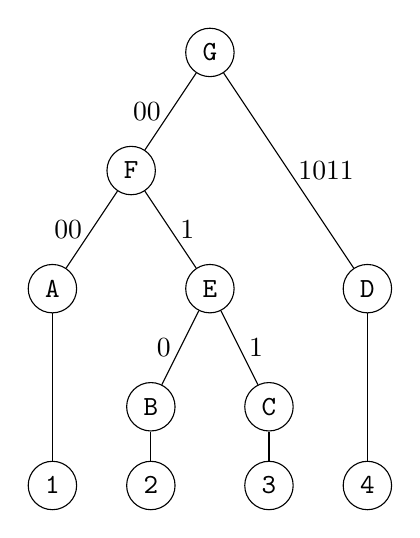
\begin{tikzpicture}
  \node[shape=circle, draw] at (-0.5,-3) (a) {\texttt{A}};
  \node[shape=circle, draw] at (-0.5,-5.5) (1) {\texttt{1}}
   edge[-] (a);

  \node[shape=circle, draw] at (.75,-4.5) (b) {\texttt{B}};
  \node[shape=circle, draw] at (.75,-5.5) (2) {\texttt{2}}
   edge[-] (b);

  \node[shape=circle, draw] at (2.25,-4.5) (c) {\texttt{C}};
  \node[shape=circle, draw] at (2.25,-5.5) (3) {\texttt{3}}
   edge[-] (c);

  \node[shape=circle, draw] at (3.5,-3) (d) {\texttt{D}};
  \node[shape=circle, draw] at (3.5,-5.5) (4) {\texttt{4}}
   edge[-] (d);

  \node[shape=circle, draw] at (1.5,-3) (e) {\texttt{E}}
   edge[-] node[left] {0} (b)
   edge[-] node[right] {1} (c);

  \node[shape=circle, draw] at (.5,-1.5) (f) {\texttt{F}}
   edge[-] node[left] {00} (a)
   edge[-] node[right] {1} (e);

  \node[shape=circle, draw] at (1.5,0) (g) {\texttt{G}}
   edge[-] node[left] {00} (f)
   edge[-] node[right] {1011} (d);
 \end{tikzpicture}
 \caption{A simple Merkle-Patricia tree with 4-bit keys. Element A is the hash of value 1, with a key of 0000. Element E is the hash of B concatenated with C, and so on recursively up to the root G. Changing any leaf value will change the root, the essential property.}
 \label{fig:Merkleexample}
\end{figure}


\subsection{The Reputation Tree}\label{sec:reptree}

The key-value pairs in the reputation tree are the reputations all users have in all skills, as well as the colony-wide totals. A single key-value pair consists of the following data:
\begin{align*}
k &=
  \begin{cases}
  \ascode{colony} & \textnormal{address of the colony the reputation is in}\\
  \ascode{user} & \textnormal{account address holding the reputation}\\
  \ascode{skill} & \textnormal{skill id of the reputation}
  \end{cases}\\
v &=
  \begin{cases}
  \ascode{amount} & \textnormal{numerical value of the reputation}\\
  \ascode{nonce} & \textnormal{unique per-leaf id (used in reputation mining)}
  \end{cases}
\end{align*}

All individual reputations are assembled into the \textbf{Reputation Tree} which is a Merkle-Patricia tree of all individual reputations in a colony, as well as the total reputation of each type held by the users in each colony. The leaves that represent these colony-wide totals are indicated by setting \ascode{user} to zero. These leaves are then inserted into the tree as described in Section \ref{sec:Merkle-summary}. We term the root hash of the resulting tree the \ascode{ReputationRootHash}, $\mathcal{RH}$.
\begin{figure}
\centering
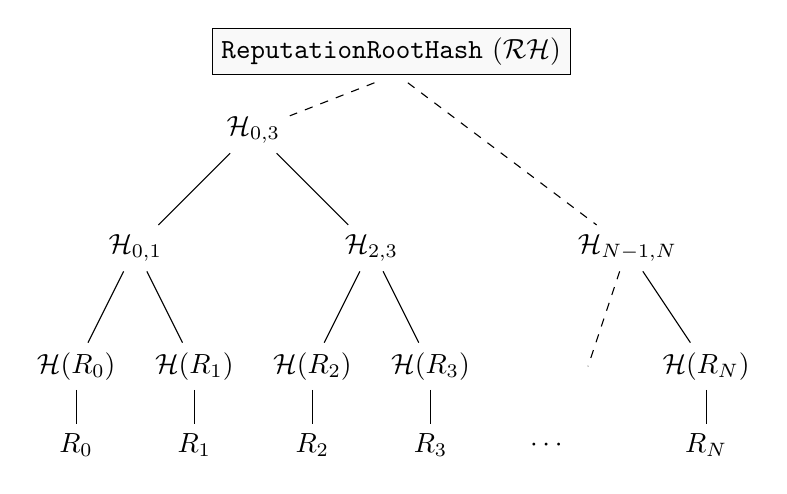
\begin{tikzpicture}
 \node at (0,-5) (r0) {$R_0$};
 \node at (1.5,-5) (r1) {$R_1$};
 \node at (3,-5) (r2) {$R_2$};
 \node at (4.5,-5) (r3) {$R_3$};
 \node at (6,-5) (rdots) {$\cdots$};
 \node at (8,-5) (rn) {$R_N$};
 %
 \node at (0,-4) (r0hash) {$\mathcal{H}(R_0)$}
  edge[-] (r0);
 \node at (1.5,-4) (r1hash) {$\mathcal{H}(R_1)$}
  edge[-] (r1);
 \node at (3,-4) (r2hash) {$\mathcal{H}(R_2)$}
  edge[-] (r2);
 \node at (4.5,-4) (r3hash) {$\mathcal{H}(R_3)$}
  edge[-] (r3);
 \node at (8,-4) (rnhash) {$\mathcal{H}(R_N)$}
  edge[-] (rn);
 %
 \node at (0.75,-2.5) (r01) {$\mathcal{H}_{0,1}$}
  edge[-] (r0hash)
  edge[-] (r1hash);
 \node at (3.75,-2.5) (r23) {$\mathcal{H}_{2,3}$}
  edge[-] (r2hash)
  edge[-] (r3hash);
 \node at (7,-2.5) (rnn) {$\mathcal{H}_{N-1,N}$}
  edge[-] (rnhash)
  edge[dashed] (6.5,-4);
 %
 \node at (2.25,-1) (r14) {$\mathcal{H}_{0,3}$}
  edge[-] (r01)
  edge[-] (r23);
 %
 \node[draw, fill=gray!5] at (4,0) (root) {\texttt{ReputationRootHash}  ($\mathcal{RH}$)};
 \node[below = 1mm of root] (dummy) {\phantom{a}}
  (dummy.north west) edge[dashed] (r14)
  (dummy.north east) edge[dashed] (rnn);
 %
 %
\end{tikzpicture}
\caption{The Merkle tree of users' reputations with \ascode{ReputationRootHash} as the root. We use $\mathcal{H}$ to indicate the \ascode{keccak256} hash function.}
\end{figure}


The \ascode{ReputationRootHash} is the only data we record on the blockchain associated with users' reputations. It summarises the state of the whole reputation system and whenever a user wishes to make use of their reputation, they can submit a Merkle proof from the reputation $\mathcal{R}_i$ they wish to make use of and ending at $\mathcal{RH}$.

\subsection{Calculating the new root hash}
To calculate the new root hash, the miners begin with the last reputation state, and decay all reputations held by all users in all colonies, in the order of the leaf nonces. They then take the set of reputation gains or losses that were not in the last state submitted, and are to be included in the next state (the update log). They apply the reputation updates to each user in each colony, updating or adding leaves as necessary (following the process described in \ref{sec:justificationTree}), to end up with a new list of reputations for all users and colonies. These new reputations are then hashed and assembled into a new Merkle-Patricia tree yielding an updated \ascode{ReputationRootHash}.

While the calculation is too large to be done on-chain due to technical and economic limitations (i.e. the block gas limit and the cost of gas, respectively), this calculation can easily be performed by a typical user's computer.

\subsection{Submission of a new root hash}
%
\subsubsection*{What is submitted?}
The final \ascode{ReputationRootHash} is submitted to the contract by the miner along with the number of leaves in the tree (\ascode{NReputationLeaves}). The miner also submits the root hash of the Justification Tree (see Section \ref{sec:justificationTree}), which will be used in the event of a dispute. These three properties uniquely identify a submission.
%
\subsubsection*{Who can submit a new root hash?}
All \rcths\ are eligible to become miners and participate in the reputation update process. Since any user can calculate the correct root hash locally, it should be possible for \emph{any} miner to submit the hash to the contract.

It is however undesirable to have too many submissions for every update. We propose a mechanism that only allows some miners to submit results to begin with. To participate in the mining process, \rcths\ must stake some of their tokens to become `reputation miners'. A submission will only be accepted from a miner if
\begin{equation*}\label{eq:mining-difficulty}
\ascode{uint256(keccak256(address, N, hash))} < \ascode{target}.\footnote{Note that internally the arguments are encoded using \ascode{abi.encodePacked} before being hashed.}
\end{equation*}
At the beginning of the submission window, the target is set to 0 and slowly increases to $2^{256}-1$ after \miningcycleduration\ hour. We limit the total number of miners allowed to submit a specific hash to 12. In the unlikely event that no submissions are received before the \miningcycleduration-hour window has elapsed, exactly one submission will be accepted, whenever it is received.

The variable $N$ that goes into the hash is some integer greater than 0 and less than the number of tokens the \rcth\ account has staked divided by \minstake\, meaning that users with a large stake have a higher chance of qualifying to submit a hash sooner than smaller stake holders. The factor of \minstake\ is introduced to ensure that all hashes a user is eligible to submit can be calculated in a few seconds by the client. It also effectively creates a minimum number of tokens that must be staked to submit a hash. This puts a tangible cost on any attacks revolving around spamming known false submissions (see Section \ref{sec:mining-possible-attacks}).

When a miner stakes, the timestamp of the stake is recorded.\footnote{If a miner adds additional stake, the timestamp is set to the weighted average of the existing and new timestamps.} In order to be eligible to submit a hash, the miner must have staked before the beginning of the current mining cycle.

\subsubsection*{Verifying a submission}
If only one state is submitted by the end of the submission period, then the new state is accepted, and proposals of the next state can begin to be made. This is expected to be the most common occurrence.

If more than one state has been submitted, then either someone has made a mistake, or there is a malicious entity trying to introduce a fraudulent reputation change. In this event, the a challenge-response protocol can establish which state is incorrect (see Section \ref{sec:challengeresponse}).

\subsubsection*{Mining rewards}

When a state is accepted, a number of (newly minted) \rcts\ are made available for the users who submitted the correct state to claim as a reward. They also receive a corresponding amount of reputation in the \rc\ (in a special mining skill, which only users in the \rc\ can earn by performing this task). This reputation update is no different from any other, aside from the limitations of who is able to earn it, and will be included in the subsequent reputation update cycle. The size of the rewards and their distribution are described in Section \ref{subsec:mining-costs-and-rewards}.

\subsection{Dealing with false submissions}\label{sec:challengeresponse}

We assume that the correct hash is one of the  submitted hashes. This is a reasonable assumption, as only one out of all the miners is required to make a correct submission, and there is an incentive for them to do so (the reward defined in Section \ref{subsec:mining-costs-and-rewards}). Thus our task is not to validate the correct hash but to invalidate the false one(s).

We must prove all but one submission incorrect by having each submission prove that they calculated more correct reputation updates before getting one wrong (if any) than another submission they are being compared against. Anyone is able to respond to a challenge (and be rewarded), regardless of who submitted the original hash; this should ensure that the correct state is always defended, even if some miners go offline.

We consider the scenario where only two submissions are made, and one is correct. In the event of more than two submissions, this same pair-wise comparison described below is repeatedly run (in parallel, where possible) among remaining submissions until only one remains.

\subsubsection{The Justification Tree}\label{sec:justificationTree}
\newcommand{\jrh}{\ensuremath{\mathbb{JRH}}}

A client submits a \ascode{JustificationRootHash} (\jrh) as part of the process of submitting a proposed new root hash. This is the Merkle root of the `Justification Tree' -- a Merkle-Patricia tree where each leaf represents not a single reputation value, but the root hash of an entire reputation state. The left-most leaf of the Justification Tree is the final accepted reputation state from the last update ($\mathcal{RH}_0$) concatenated with the number of leaves ($\mathcal{L}_0$) in the reputation tree $\mathcal{RH}_0$ is the root of. The right-most leaf of the Justification Tree is the \ascode{ReputationRootHash} they submitted ($\mathcal{RH}_N$) concatenated with the number of leaves it contains ($\mathcal{L}_N$). We denote these leaves as $\mathcal{RH}_0 \cdot \mathcal{L}_0$ and $\mathcal{RH}_N \cdot \mathcal{L}_N$.

The intermediate leaves represent the evolution of the global reputation state after applying some subset of the full sequence of reputation updates required. Each state represented by a leaf differs from the reputation states in neighboring leaves in \textit{at most} a single reputation.\footnote{It is possible for two adjacent leaves to be identical if the reputation update the transition between them represents does not result in a change in reputation -- e.g. a reputation loss in a reputation that is already zero.} In order to do this in a consistent way, we must order all the updates in a reputation cycle. The canonical ordering for reputation updates is:

\begin{enumerate}
\item All decays of existing reputations, in order of \ascode{nonce},
\item The entries in the reputation update log, in order of appearance in the reputation update log. A single one of these entries corresponds to at least two reputation updates with an unbounded upper limit (since there can be many parent and child updates). These updates are themselves ordered:
\begin{enumerate}
  \item Colony-wide total of any impacted child reputations \label{lab:colonyWideChildren}
  \item Colony-wide total of any impacted parent reputations \label{lab:colonyWideParents}
  \item The colony-wide total of the origin reputation
  \item User-specific child reputations \label{lab:userChildren}
  \item User-specific parent reputations\label{lab:userParents}
  \item User-specific origin reputation
\end{enumerate}
The origin reputation is defined to be the skill specified in the reputation log where the reputation is to be lost or gained. Where multiple child reputations are required to be updated as part of \ref{lab:colonyWideChildren} or \ref{lab:userChildren}, they are done so in the order they appear in the \ascode{children} property of the origin skill. Where multiple parent reputations are required to be updated as part of \ref{lab:colonyWideParents} or \ref{lab:userParents}, the immediate parent is updated first, then the immediate parent of that skill, and so on until no parents remain. We do the decay calculations first to give users the benefit of the doubt during reputation updates so they do not lose reputation they have only just earned to premature decay.
\end{enumerate}

As a miner applies the reputation updates for a cycle in this order, they should take each intermediate \ascode{ReputationRootHash} values and build the Justification Tree by adding the intermediate \ascode{ReputationRootHash} values concatenated with \ascode{NReputationLeaves} to the tree, \textit{with key equal to the update number}, starting from 0. Note that unlike in the Reputation Tree, the keys should not be hashed. This will become important further on in the dispute process, as we will need to be able to identify sequentially adjacent reputation updates. The intermediate leaves of the Justification Tree represent the evolution of the reputation state, with $\mathcal{RH}_i$ corresponding to the reputation state after the first $i$ reputation updates in this cycle have been applied. An example of such a tree is shown in Figure \ref{fig:justification-tree}.

 %
\begin{figure}
\centering

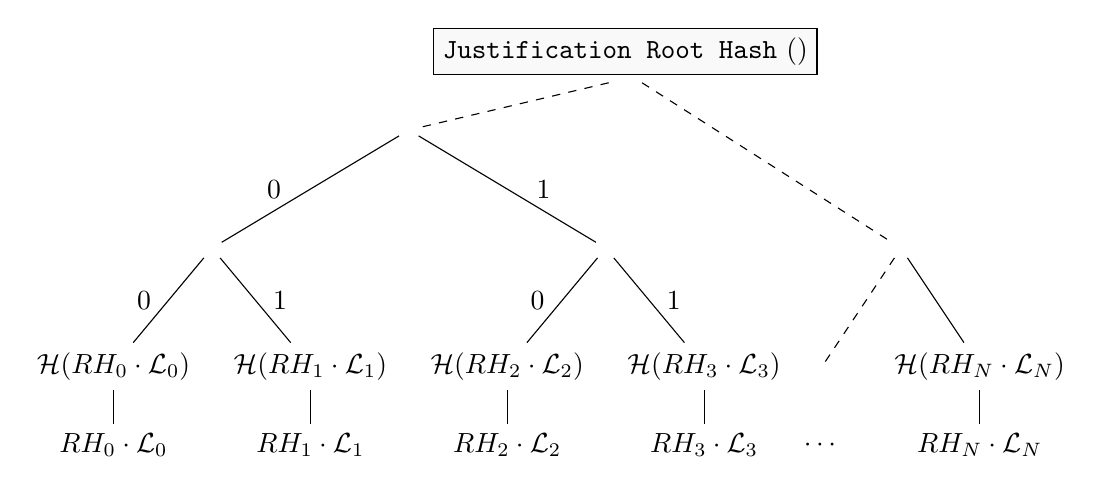
\begin{tikzpicture}
 \node at (0,-5) (r0) {$RH_0\cdot \mathcal{L}_0$};
 \node at (2.5,-5) (r1) {$RH_1\cdot \mathcal{L}_1$};
 \node at (5,-5) (r2) {$RH_2\cdot \mathcal{L}_2$};
 \node at (7.5,-5) (r3) {$RH_3\cdot \mathcal{L}_3$};
 \node at (9,-5) (rdots) {$\cdots$};
 \node at (11,-5) (rn) {$RH_N\cdot \mathcal{L}_N$};
 %
 \node at (0,-4) (r0hash) {$\mathcal{H}(RH_0\cdot \mathcal{L}_0)$}
  edge[-] (r0);
 \node at (2.5,-4) (r1hash) {$\mathcal{H}(RH_1\cdot \mathcal{L}_1)$}
  edge[-] (r1);
 \node at (5,-4) (r2hash) {$\mathcal{H}(RH_2\cdot \mathcal{L}_2)$}
  edge[-] (r2);
 \node at (7.5,-4) (r3hash) {$\mathcal{H}(RH_3\cdot \mathcal{L}_3)$}
  edge[-] (r3);
 \node at (11,-4) (rnhash) {$\mathcal{H}(RH_N\cdot \mathcal{L}_N)$}
  edge[-] (rn);
 %
 \node at (1.25,-2.5) (r01) {}
  edge[-] node[left=1mm] {0} (r0hash)
  edge[-] node[right=1mm] {1} (r1hash);
 \node at (6.25,-2.5) (r23) {}
  edge[-] node[left=1mm] {0} (r2hash)
  edge[-] node[right=1mm] {1} (r3hash);
 \node at (10,-2.5) (rnn) {}
  edge[-] (rnhash)
  edge[dashed] (9,-4);
 %
 \node at (3.75,-1) (r14) {}
  edge[-] node[left=2.5mm] {0} (r01)
  edge[-] node[right=2.5mm] {1} (r23);
 %
 \node[draw, fill=gray!5] at (6.5,0) (root) {\texttt{Justification Root Hash}  (\jrh)};
 \node[below = 1mm of root] (dummy) {\phantom{a}}
  (dummy.north west) edge[dashed] (r14)
  (dummy.north east) edge[dashed] (rnn);
 %
 %
\end{tikzpicture}
\caption{The Justification Tree. The leaf containing $\mathcal{H}(RH_0\cdot \mathcal{L}_0)$ -- the last accepted reputation state -- is found at key \ascode{...00}. The leaf containing $\mathcal{H}(RH_1\cdot \mathcal{L}_1)$ -- the reputation state with the decay of the existing skill with nonce 0 applied -- is found at key \ascode{...01}. Every intermediate state is recorded in the tree up to $\mathcal{H}(RH_N\cdot \mathcal{L}_N)$, which is the proposed new reputation state with all reputation updates applied.}
\label{fig:justification-tree}
\end{figure}

\subsubsection{Resolving a dispute}

If a dispute occurs, the first step is for each submission to verify the Justification Tree they submitted alongside their proposed new root hash.

\subsubsection*{1. Verifying the Justification Tree}

For a justification tree to be deemed valid, it must:

\begin{itemize}
\item Have $\mathcal{H}(RH_0 \cdot \mathcal{L}_0)$ at key 0,
\item Have $\mathcal{H}(RH_N \cdot \mathcal{L}_N)$ at key $N$,
\item Have a plausible structure.
\end{itemize}

The first two items are relatively straightforward to prove via Merkle proof. The last requirement requires slightly more explanation. A Justification Tree with two leaves could meet the first two requirements, but we would be able to tell this tree wasn't plausible as a Justification Tree because the Merkle proofs supplied to prove the first two requirements would not be of the expected length.\footnote{We know that every reputation cycle will at least have log entries for rewarding those who submitted the previous reputation state successfully.} This length is calculable because we know how many leaves are meant to be in the tree and what keys they are expected to be at (every key between 0 and $N$). We are also able to determine the branchmasks that these proofs should have (the binary representations of $2^{\lceil\log_2 (N+1) \rceil} - 1$, and $N$ respectively), which further constrains the shape of a plausible tree.

Unfortunately, based on these two proofs, we are unable to guarantee the Justification Tree contains a leaf at every key from 0 to $N$. This is because we do not know how many leaves the siblings used in the Merkle proofs contain, and it is not feasible to request a proof for every key between $1$ and $N-1$. This is why the constraint is limited to being `plausible'. With the approach we have taken, however, we are at least able to guarantee that key $N$ is the last in the Justification Tree, that key $0$ is the first (though this is a trivial consequence of it existing), and there are at least some number of other keys in the tree.\footnote{This number is $\lceil\log_2 (N+1) \rceil + \#_{1}(N) - 2$, where $\#_{1}(N)$ is the binary logarithm of the $N$th integer in Gould's sequence. To derive this expression, consider how many siblings each proof requires; each sibling corresponds to at least one other key. In our case, $\#_{1}(N)$ provides the number of set bits in the branchmask of the proof for key $N$ i.e. how many siblings that the Merkle proof of key $N$ has. The $-2$ accounts for the key-value pairs stored at 0 and $N$.}

Since any two differing submitted states agree on the first leaf $\mathcal{RH}_0$ (the \ascode{ReputationRootHash} accepted at the end of the previous iteration of the mining cycle), and disagree on the last leaf $\mathcal{RH}_N$ (the hash they submitted), there must be a hash $\mathcal{RH}_i$ that they agree on, and a hash that $\mathcal{RH}_{i+1}$ that they do not. This is a reputation update where they agree on the starting state but disagree on the result. This transition is meant to be the effect of a single reputation update (the $i^{th}$), and this is the reputation update we will calculate on-chain to establish which submission is incorrect.\\

\noindent First, however, we must establish where the two submissions begin to differ.

\subsubsection*{2. Searching for the discrepancy}
The contract requires both parties to submit repeated Merkle proofs to locate $\mathcal{RH}_{i+1}$, the first disagreement hash. We shall call the two parties $A$ and $B$ and we shall indicate which party made a submission by a superscript of $A$ or $B$. Furthermore we introduce the simplifying notation of $\overline{h}$ to mean `sibling of $h$' in the Merkle tree.

Along with their justification root hashes $\jrh^A$ and $\jrh^B$ both parties have already submitted proofs for the left-most leaf. Ignoring the branchmasks for simplicity, these proofs have the form:
\[
 \overline{\mathcal{RH}_0}^A, \overline{h_{0,1}}^A, \overline{h_{0,2}}^A, \ldots \overline{h_{0,2^k}}^A \qquad \textnormal{ terminating at } \jrh^A
\]
and
\[
 \overline{\mathcal{RH}_0}^B, \overline{h_{0,1}}^B, \overline{h_{0,2}}^B, \ldots \overline{h_{0,2^k}}^B \qquad \textnormal{ terminating at } \jrh^B
\]
where $k$ is the largest integer such that $2^k$ is smaller than $n$.

When the first miner (say $A$) submits their proof the contract saves the values of $h_{0,2^k}^A$ and $\overline{h_{0,2^k}}^A$. When the second miner submits their proof the contract compares $h_{0,2^k}^A$ to $h_{0,2^k}^B$. If they are not equal, the contract saves both of these values (and forgets $\overline{h_{0,2^k}}^A$). If they are equal, the contract retains the values of $\overline{h_{0,2^k}}^A$ and $\overline{h_{0,2^k}}^B$ (forgetting $h_{0,2^k}^A$).

The rationale behind this behaviour is the following: If $h_{0,2^k}^A = h_{0,2^k}^B$ then the two justification trees are equal between $\mathcal{RH}_0$ and $\mathcal{RH}_{2^{k-1}}$ and the first discrepancy must lie in the right-hand subtree whose root is $\overline{h_{0,2^k}}^A$ for miner $A$ and $\overline{h_{0,2^k}}^B$ for miner $B$. If on the other hand $h_{0,2^k}^A \neq h_{0,2^k}^B$, then the first discrepancy must lie in the left-hand subtrees given by $h_{0,2^k}^A$ and $h_{0,2^k}^B$. The situation is summarised by
\begin{eqnarray*}
 h_{0,2^k}^A \neq h_{0,2^k}^B & \Longrightarrow & \textnormal{First discrepancy occurs at some } \mathcal{RH}_i \textnormal{ with } 0 \leqslant i < 2^k\\
 h_{0,2^k}^A = h_{0,2^k}^B & \Longrightarrow & \textnormal{First discrepancy occurs at some } \mathcal{RH}_i \textnormal{ with } 2^k \leqslant i < n
\end{eqnarray*}

The contract begins its search by %pseudorandomly%\footnote{This pseudorandomness is to help mitigate an attack described in Section \ref{sec:mining-possible-attacks}.}
%picking an index $j$ from within the range the first discrepancy in known to lie in. It then
%
picking an index $j$ from within the range the first discrepancy in known to lie in (say always the smallest), and requiring both parties to provide a Merkle proof showing value of \ascode{ReputationRootHash} and \ascode{NReputationLeaves} at that key in the Justification Tree. The required target of this proof is no longer the $\jrh$ itself, but rather the retained value for $h_{0,2^k}$ or $\overline{h_{0,2^k}}$.

The process as before of comparing hashes and retaining the roots of either the left-side subtree or the right-side subtree is repeated. With each iteration, the range of possible values for the index of the first discrepancy is reduced by (on average) a factor of two and the length of the required Merkle proofs is reduced by at least one.

There are two ways this process can terminate. The first way the process terminates is when one party does not respond to a challenge in adequate time, either because they could not or chose not to. In this case the party not responding is deemed to be incorrect. The other way the process terminates is when it has reached the bottom of the tree and determined $i$, the disputed reputation update.

\subsubsection*{3. Confirming $i$ }

Once the contract has found the index $i$ such that $\mathcal{RH}^A_{i}=\mathcal{RH}^B_{i}$ but $\mathcal{RH}^A_{i+1}\neq\mathcal{RH}^B_{i+1}$, the contract then requires each party to submit the value stored at the key $i+1$ in the Justification Tree to confirm that it is there. It is possible that this was already done during the binary search, but it is not guaranteed. The value of the \ascode{ReputationRootHash} and \ascode{NReputationLeaves} at this key are stored in the contract managing the dispute resolution. Again, if one party does not respond in time, they are assumed to be incorrect.

\subsubsection*{4. Deciding which submission performed the correct calculation}

In most cases, only one of the two submissions will be able to perform the transaction corresponding to this step. There are several types of calculation and checks that might need to take place, depending on which transition the two submissions first disagree on, and the values of \ascode{ReputationRootHash} and \ascode{NReputationLeaves} they placed in their Justification Trees. All of the following must be performed on chain to verify the calculation under dispute.

\begin{itemize}
\item \textbf{Check the key} As part of the Merkle proofs submitted (see the next step), the \ascode{key} of the reputation under dispute is submitted. This is a concatenation of the colony address the reputation is in, the skill the reputation is in, and the account address holding the reputation (which is possibly the zero address if the total reputation in the colony is under dispute). Based on the value of $i$, which has already been established during the binary search, and the known canonical ordering of reputation updates, the contract is able to check these values. In the case where the update under dispute is due to a log entry (as opposed to normal decay), the index of the log entry under dispute is supplied by the user and verified on-chain, to avoid iteration over the unbounded log.
\item \textbf{Check the claimed before and after values} The values of the reputation at \ascode{key} in $\mathcal{RH}_{i}$ and $\mathcal{RH}_{i+1}$ for the submission in question are proved via Merkle proof. If it is claimed an existing reputation is being updated, then the proofs' siblings and branchmask are required to be the same to guarantee no other reputations have been changed. If a new reputation is claimed to be being added (indicated by $\mathcal{L}_{i+1} - \mathcal{L}_i = 1$), the proof for the reputation in $\mathcal{RH}_i$ is not required as the reputation should not be in the tree, but an additional check will be performed later to confirm this.
\item \textbf{Perform the calculation} This has two elements. The first is to check that the \ascode{nonce} for the reputation has not changed in the leaf if an existing leaf is being updated. If a new leaf is being added, the value of the \ascode{nonce} is checked to be one larger than the $\mathcal{L}_{i}$ that they have provided (as each \ascode{nonce} is given in sequence). The second is to check that the value of the reputation is correct. It can be a decay, or an update due to an entry in the log, the potential consequences of which are described in section \ref{sec:calculating-reputation-updates}.
\item \textbf{Additional checks} Depending on the type of update being disputed, additional checks may be required
\begin{enumerate} \item Any additional reputation values needed for the calculation are proved to be in $\mathcal{RH}_{i}$ (which both parties agree on the value of) as required via Merkle proof. The canonical ordering of reputation updates ensures that any values required for the calculation under dispute are present in $\mathcal{RH}_{i}$ and have not yet been altered by the log entry under consideration.
\item Similarly, if a new leaf is added, a Merkle proof for the reputation in $\mathcal{RH}_{i}$ with the previous \ascode{nonce} is checked to confirm the \ascode{nonce} assigned to the new node is plausible.
\item If during the calculation, the user claims that a reputation they need for a calculation does not exist in $\mathcal{RH}_{i}$, and so they will use a value of 0, they must prove it does not exist in the tree.\footnote{They do this by providing a Merkle proof for an existing reputation in $\mathcal{RH}_{i}$ whose hashed key has the longest shared prefix with the hashed key of the reputation being added. By examining the branchmask of this proof, and the (hashed) keys of the proved reputation and the reputation being claimed to not exist, the contract is able to confirm the latter does not exist in $\mathcal{RH}_{i}$. If a key with a shorter shared prefix is used, the branchmask will already contain a branch point where they diverge and this proof will fail.} % I don't feel like I've explained this very well. Perhaps it warrants a subsection somewhere?
\item If a new reputation value is being added to the tree, we also prove that the reputation that it ends up closest to in the tree exists in $\mathcal{RH}_{i}$. We are therefore able to deduce what the proof for that reputation in $\mathcal{RH}_{i+1}$ should be if only the new leaf is added. By checking this Merkle proof is valid, we ensure no other changes have been made to the reputation tree.
\end{enumerate}
\end{itemize}

It is possible that both submissions will successfully submit the transaction that validates their submissions as described here. This can happen when a new leaf is being added, and the submissions have disagreed over the \ascode{nonce} the reputation should be given. Whichever has successfully awarded the highest \ascode{nonce} is deemed the correct submission. If neither party responds to a particular stage in this process in time, both are eliminated from consideration.

If the \miningcycleduration-hour mining cycle window has not elapsed by the time only one submission remains, the next window only opens when the current window has elapsed. If the \miningcycleduration-hour window has elapsed by the time the dispute process has finished, the next submission window opens immediately.

\subsection{Calculating reputation updates}\label{sec:calculating-reputation-updates}
% TODO: I think this needs to be moved to before 'Dealing with false submissions'.

\subsubsection{Keeping track of reputation changes}

Fundamentally, there are two types of reputation update that occur:
\begin{itemize}
 \item Decay of existing reputation.
 \item Addition or removal of reputation as a reward or punishment.
\end{itemize}

When a user earns reputation in a skill or domain, they also earn reputation in all parent domains, which corresponds to $2\times\left(\ascode{n\_parents}+1\right)$ reputation updates. Alternately, when a user loses reputation, they also lose reputation in all parents and all children representing a total number of updates of $2\times\left(\ascode{n\_parents} + \ascode{n\_children} + 1\right)$. The factors of two here come from also updating the relevant colony-wide totals.

In Section \ref{subsec:on-chain-representation-of-skills}, we asserted we store \ascode{n\_parents} and \ascode{n\_children} for all skills and domains. It is only by having access to the number of parents and children for each reputation and the reputation update log recording how many reputations have been updated already in this update cycle (via \ascode{n\_updates}) that the resolution protocol is able to perform the binary search of the justification trees submitted by the disagreeing users. At the start of the challenge protocol, the contract can look up the last entry in the update table for the cycle under consideration, and work out how many updates have occurred in this cycle based on the number of updates prior and the number of parent and child reputations. After verifying that both submitted justification trees contain this exact number of leaves it can proceed to the binary search.

If the discrepant transition is a decay transition they must also supply a Merkle proof that the starting value assumed for the user corresponds to the value that user had at the end of the last update cycle. A decay transition is identified by the Merkle path corresponding to an index in the justification tree smaller than the number of leaves in the reputation tree at the end of the last successful update.

\subsubsection{Earning reputation for the first time}\label{sec:earning-rep-for-first-time}
When a user earns reputation in a new skill, at least one new leaf is added to the tree --- if they have not earned reputation before in some of the parents, then they will also cause further new leaves to be added. Additional new leaves will be added if they are the first user in a colony to earn those particular skills, making the total reputation for that skill in the colony non-zero. During a dispute, when the user proves that they have included the update in the tree, it is not possible to check (efficiently) on-chain that they should not have added it to an existing leaf instead. However, because during the resolution process we are always comparing two submissions against each other, one of two things will be true:\footnote{Assuming that one of the two submissions is correct.}
\begin{itemize}
 \item Both submissions added a new leaf to the tree. If there was a discrepancy, then it is in the maths conducted on this leaf, not the addition of the leaf itself. The maths can be checked on-chain to establish which result is correct.
 \item One submission adds the new reputation to an existing leaf (the correctness of which can be checked on-chain easily). In this case, the user who added the leaf incorrectly is wrong.
\end{itemize}

\subsubsection{Transfers of reputation between accounts}\label{sec:reptransfer}

The most important quality of reputation that distinguishes it from a token is that it is tied to an account and cannot be transferred. However, in the event of disputes (Section \ref{sec:objections-and-disputes}) it can happen that one party to a dispute loses reputation while the other gains. This process has to be modelled as a `reputation transfer' to ensure that reputation is never created in this process (i.e. the reputation lost by the loser is at least as much as the reputation gained by the winner).

If an entry in the reputation update log indicates that a dispute has occurred and been resolved, then there will be a number of transfers of reputation between users represented by a single entry. Each such transfer will have to accommodate the updates of all the parents of the reputation being gained by one user, and updates of all the parents and children of the reputation being lost by the other. However, we have to ensure that the user who is losing reputation still has the reputation to lose if another user is gaining it.

To achieve this, all the transactions that correspond to updating the reputations of the user gaining the reputation are done first. In the event such a transaction must be proved to be correct in the resolution protocol, the users can provide a proof of the losing user's reputation, prior to them losing it in this event in update cycle, and this can be compared to the amount of reputation intended to be gained. Whichever is smaller is used as the amount of reputation the user is gaining during the calculations.

Then, when calculating the reputation deduction to be applied to the losing user, the reputation that was used as the voting weight should be done last i.e. all the children and parents should be considered first, as it is the amount of the reputation that was eligible to vote that will determine the fraction lost of each of the child reputations. %If any of these calculations need to be proved correct during the resolution protocol,

For further details about reputation transfers and disputes, see Appendix \ref{appendix:rep-transfer}.

\subsubsection{The reputation decay calculation}\label{sec:repdecay}
The reputation decay process was described above as being continuous. In practise, it will decay by a small, discrete amount during each reputation update cycle following an exponential decay. However, such a calculation is not possible to do accurately on-chain during the resolution protocol, so we must use an approximation. The details of the approximation we use, and a proof that this approximation is accurate and will not affect the running of (active) colonies can be found in Appendix \ref{appendix:rep-decay}.

\subsection{Denial of service attacks}\label{sec:mining-possible-attacks}

In the event of multiple submissions, finding the correct one takes time --- the timeout $t$ for the challenge-response must be reasonable to allow the transaction defending a submission to propagate and be mined. A denial-of-service attack is therefore possible, whereby an attacker makes many false submissions. However, if these false submissions were random hashes, unable to be defended, then none would be defended correctly within the first timeout window, and the attack would quickly end. For pairings where neither submission is defended, any user can remove both submissions from consideration and claim the tokens that were staked to allow submission.

The denial of service attack (to delay a proper reputation update) can only be sustained when the false submissions are incorrect only in some leaves, and the majority of the justification tree is correct. In this scenario, the attacker successfully defends each of their submissions for as long as possible to delay the resolution of the reputation mining protocol as much as possible.

Any such attack is capped by the first round of pairings of submissions against each other. Even if the attacker made millions of submissions, only a finite number of those would be able to be successfully defended due to the block size --- currently, no more than 4500 submissions would be able to be defended, even if the attacker used up all block space during the timeout.\footnote{These figures assume $1.5\pi\times10^6$ gas in a block, and that each transaction is only 21000 gas for a worst-case-scenario calculation.} With only 4500 submissions able to make it to the second round, the length of time the DoS attack would be sustained for is given by

$$t \times \left\lceil\log_2\left(4500\right)\right\rceil\times \left\lceil\log_2\left(N_{\rm updates}\right)\right\rceil$$

\noindent where $N_{\rm updates}$ is the number of reputation updates that have been made in this update cycle. To arrive at this figure, we know there will need to be $\left\lceil\log_2\left(4500\right)\right\rceil$ rounds of comparison between submissions to eliminate all but one. Each round will require $\left\lceil\log_2\left(N_{\rm updates}\right)\right\rceil$ interrogations of the justification tree to establish where the two submissions being compared differ. Finally, each interrogation can take up to $t$ before it is considered to have timed out and one or both of the submissions is deemed invalid. The product of these three factors tells us how long this reputation update can be delayed by an attacker.

Long term, $N_{\rm updates}$ will be dominated by the decay transactions rather than by any updates that have occurred since the last reputation state was established. Even if the Colony Network were wildly successful, with 100000 colonies, each with 1000 users that had earned some reputation in 1000 different skills in each of the structural and skill hierarchies, and using 5 minutes as the value of $t$, the delay to the reputation updates would only be around $36$ hours. Recent congestion on the Ethereum network has shown that we will need to be able to accommodate situations where block space is at a premium; the reputation mining client will need to recognise when this is occurring, and send transactions with higher gas prices as appropriate in order to meet the timeout deadline.

There would be little effect on the rest of the Colony Network in this time. Users would still be able to exercise their reputation from the previous reputation update, and continue to influence decisions with that reputation. Indeed, this shows what perhaps the main motivation for such an attack would be --- if a user knew that they had been `caught' behaving badly, and was due to lose all their reputation, they might try such an attack to eke out the last bits of influence they possibly could. However, decisions in the Colony network do not resolve quickly, and in a well-developed colony we would not expect any one person to have a large amount of reputation when compared to the rest of the colony. It therefore seems unlikely any one user would be able to unduly influence decisions significantly while conducting such an attack.

Assuming this attack continued, then the reputation mining protocol would effectively only update every 36 hours. Users staking would become more susceptible to variance in terms of the rewards, but otherwise little would change in the day-to-day functioning of any individual colony.

However, the attacker would lose \emph{all} the \rct\ that they had staked (which would be around 4500 times the expected minimum stake) in order to perform the attack, and so would have to buy more to attack again making this attack exceedingly expensive.


Note: There is an edge case to consider in which the attacker is sending enough defending transactions to completely fill the blocks. In such a case however we assume that the defence of the legitimate state is always successfully included in block, as a one-off increase in gas costs will always be worthwhile to ensure the legitimate state is defended. Between now and the deployment of the Colony Protocol, we will carefully observe the Ethereum network to gather empirical data about the cost and practicability of such an attack and will adjust the timeout parameter $t$ accordingly. Longer timeout periods make this attack exceedingly difficult and expensive, but would also slow down the resolution protocol.

\subsection{Costs and rewards of mining}\label{subsec:mining-costs-and-rewards}
In order to be involved in the reputation mining process, \rcths\ must stake their tokens with the Colony Network Contract. This allows them to submit a reputation hash as part of the reputation mining process described above.

If they submit a new hash, this is recorded and they are noted as the first account to submit that hash. If they submit a hash that has already been submitted, they are appended to a list of users that have submitted that hash. The system allows for a maximum of 12 miners to be added to the list in each round. The same miner is allowed to appear on the list multiple times, but using different values of $N$ in the inequality \eqref{eq:mining-difficulty} on page \pageref{eq:mining-difficulty}.

If a hash is found to be incorrect, all those who submitted it lose some of their stake. If a hash is deemed correct, however, the miners who submitted it gain \rcts\ and reputation.

The total amount of reputation earned by miners is not fixed, but varies along with activity in the \rc. The system tries to ensure that on average, 25\% of \rc\ reputation comes from mining. %In times of growing activity, more reputation will go to tasks and in times of declining activity more reputation will go to the miners.

Suppose that the reputation earned in the \rc\ every hour due to all activity (mining included) is constant at $h$, then eventually the colony will reach a steady state in which the decay of reputation is balanced out precisely by the newly earned reputation and
\begin{equation}
 R_{tot} \left( 1 - e^{-k} \right) = h
\end{equation}
\noindent where $k$ is the decay constant used in each update period (see Appendix \ref{appendix:rep-decay}) and $R_{tot}$ is the total reputation in the \rc. If one quarter of all reputation is to come from mining, then the hourly mining reward $M$ in this situation should be given by
\begin{equation}\label{eq:mining-reward}
 M = \frac{h}{4} = \frac{R_{tot} \left( 1 - e^{-k} \right)}{4}.
\end{equation}

The \emph{actual} mining rewards are calculated based on the above model and we \emph{define} the total reputation to be earned by miners in a given hour to be given by equation \eqref{eq:mining-reward}.

Miners who make a submission in a given reputation update cycle are entitled to a share of this reward. When a miner makes their submission, their weighting for that submission is calculated and recorded, and this is added to the total weights of all submitters for this hash so far. The $n^{th}$ submitter has a weight of
\begin{equation}\label{eq:miner-weighting}
 w_n = \left(1 - \exp\left(\frac{-t_n}{T}\right)\right) \times \left( 1 - \frac{n-1}{N} \right)
\end{equation}
where $t_n$ is a number of seconds that the $n^{th}$ miner has staked their tokens for and $T$ and $N$ are normalising constants. $T$ is set to a number of seconds representing \miningstakeduration\ days, and $N$ is set to twice the length of the list of submitters --- in our case $N=24$.

The first factor in equation \eqref{eq:miner-weighting} encourages users to stake their tokens for long periods of time when they register as miners. When locking tokens for $T$ seconds, this first factor grows to 0.63, when locking for $2T$ it grows to 0.86, and the factor approaches 1 as the locking time approaches infinity. The second factor in equation \eqref{eq:miner-weighting} encourages miners to submit the hash as soon as possible, with this factor becoming smaller the later users submit; the first submission will have twice the weight of the last submission, all other factors being equal.

Once the submission window has expired, and either there was only one submitted hash, or all but one submitted hash has been proved to be wrong, any user can make a transaction to make this submitted hash the canonical reputation state used by the network until the end of the next update cycle. This transaction mints and transfers the CLNY reward to the miners, as well as adds reputation changes for the miners to the start of the reputation change log, where they will be included in the next update cycle.

The reward earned by each miner on the list is given by
\begin{equation}\label{eq:miner-payout}
 m_n = M \frac{w_n}{W} \quad \textnormal{where} \quad W = \sum_{n=1}^{12} w_n
\end{equation}
i.e. the mining reward $M$ is divided among the miners according to their relative weighting.

\subsection{Emergency shutdown}\label{sec:big-red-button}

Section \ref{sec:escape-hatches} described a transaction from a whitelisted account can put a colony into `recovery mode' during which the state can be edited, the effects of bugs can be corrected and upgrades can be made. Similarly, the reputation mining process will also have an emergency stop-and-repair mechanism (to begin with). This will allow the whitelisted accountes to revert the reputation root hash to a previous version and halt all updates to the reputation state until the issues have been resolved (which will likely involve a contract upgrade). The colonies will be able to continue operations as usual using the reputations of the last valid state, which will be temporarily frozen and not decay.

\newpage


\section{Finance: Managing Funds and Bounties}\label{sec:finance}
This section deals with the mechanisms by which a colony \emph{allocates} financial resources to domains and tasks. The norm is for resources to be allocated from the general to the particular, and that all allocations with sufficient reputational `backing' may proceed without a vote. As long as there is no disagreement, everything will run smoothly and automatically.

For how revenue earned by a colony is handled see Section \ref{sec:revenue}.

\subsection{Tokens and Ether}
Every colony has its own ERC20-compatible token. These tokens are under the control of the colony contract and may be used to pay for work done in the colony. Tokens only leave the control of the colony upon being paid out for completed tasks.\footnote{Currently, the only way this rule can be broken is by the Colony conspiring to abuse the Arbitrary Transaction feature described in Section \ref{sec:arbitrary-transaction}. }

To pay out tasks, in addition to local tokens, a colony may also use Ether, CLNY and other ERC20 tokens that have been explicitly whitelisted by the Colony Network.


\subsection{Funding pots and funding proposals}\label{sec:pots-and-fp}
All tokens and currencies are administered by the colony contract; it is responsible for all the bookkeeping and allocations.

\textbf{Each domain and each task in a colony has an associated \emph{funding pot}.} A funding pot can be thought of as acting like a wallet specific to a particular domain or task. To each funding pot, the colony contract may associate any number of unassigned tokens it holds. Depending on context, the funds in a funding pot may be referred to as the bounty, the budget, the salary or working capital. In addition to the funding pots, there is a special \emph{rewards pot} which accumulates tokens to be distributed to members as \textit{rewards} (see Section \ref{sec:revenue}).

\textbf{Funds are transferred between pots through \emph{funding proposals}.}
\begin{description}
 \item A Funding Proposal consists of the following data:
 \begin{itemize}
  \item \ascode{\textbf{Creator}}	--	The person that created the proposal.
  \item \ascode{\textbf{From}}	--	Funding pot funds are coming from.
  \item \ascode{\textbf{To}}	--	Pot funds are going to (may be the rewards pot).
  \item \ascode{\textbf{TokenType}}	--	The token contract address (0x0 for Ether).
  \item \ascode{\textbf{CurrentState}}	--	The state of the proposal (i.e. inactive, active, completed, cancelled).
  \item \ascode{\textbf{TotalPaid}}	--	How much has been transferred along this funding proposal so far.
  \item \ascode{\textbf{TotalRequested}}	--	The maximum amount to transfer after which this funding proposal is considered `completed'.
  \item \ascode{\textbf{LastUpdated}}	--	The time when the funding proposal was last updated.
  \item \ascode{\textbf{Rate}}	--	Rate of funding.
  \item \ascode{PunishCreator} -- Whether the creator should be punished upon completion.
 \end{itemize}

\end{description}
We distinguish between two types of funding proposals: Basic Funding Proposals (BFP) intended for normal use, and Priority Funding Proposals (PFP) intended to be used when atypical circumstances present themselves. The basic funding proposal may start funding the target straight away, whereas a priority funding proposal must be explicitly voted on before it starts directing funds. Furthermore, for a basic funding proposal the target pot must be a direct descendant of the source in the hierarchy whereas a priority funding proposal has no such restrictions.

Priority funding proposals should be used when funds need to be directed somewhere that is not a direct descendant of the source, when the funding rate needs to be very high (including immediate payment), or when the funding rate should be otherwise controlled (e.g. in the case of paying a salary).

For either funding proposal, the assignment to funding pots associated with domains or tasks is purely a bookkeeping mechanism. From the perspective of the blockchain, Ether and tokens are held by the colony contract until they are paid out when a task is completed.

\subsubsection{Creating a funding proposal}
Any member of the colony may create a funding proposal. The proposer must have 0.1\% of the reputation of the domain that is the most recent common ancestor of the source and target pots. They must stake an equivalent fraction of the colony's tokens. This stake is used to help discourage spamming of funding proposals and provide a mechanism whereby the creator can be punished for bad behaviour.

\subsubsection{From, To and TokenType}
The purpose of a funding proposal is to move tokens of \ascode{TokenType} from a pot \ascode{From} to a pot \ascode{To}.

The \ascode{TokenType} may be any ERC20 token whitelisted for use in the network, Ether, CLNY or the Colony's own Token. The \ascode{From} field must be a funding pot associated with a domain or a task in the colony, while the \ascode{To} field must be either a funding pot or the special rewards pot. If the funds are to move `downstream' from a domain to one of its children, a basic funding proposal is often sufficient.

\subsubsection{CurrentState}
The state of a funding proposal is either \ascode{inactive}, \ascode{active}, \ascode{completed} or \ascode{cancelled}. Only an active funding proposal is in line to channel funds. A basic funding proposal begins in active state while a priority one begins inactive (i.e. it must be activated by a vote). A funding proposal is completed when its \ascode{TotalPaid} reaches \ascode{TotalRequested}. Any other state changes must be made through the dispute mechanism (see Section \ref{sec:objections-and-disputes}).

\subsubsection{TotalPaid and TotalRequested}
The total number of funds that a funding proposal wishes to reallocate is called its \ascode{TotalRequested} amount. Due to the mechanism by which funding proposals accrue funds over time, it is common that a funding proposal will have received a part but not all of its \ascode{TotalRequested} amount. The total number of tokens accrued to date are stored in its \ascode{TotalPaid} amount.

\subsubsection{Rate and LastUpdated}
When a funding proposal is eligible to accrue funds (see Section \ref{subsec:funding-queue}) it does so at a specific \ascode{Rate}. Since nothing happens on the blockchain without user interaction, the funding system uses a form of lazy evaluation. To claim funds that the proposal is due, a user may `ping' the proposal --- i.e. the user manually requests an update. When pinged, the time since \ascode{LastUpdated} is multiplied by the \ascode{Rate} to determine how many tokens the proposal would have accrued in the interim if funding flow were continuous. This amount is added to \ascode{TotalPaid} and the current time is recorded as \ascode{LastUpdated}.

\ascode{TotalPaid} is only ever increased up to \ascode{TotalRequested} and when this happens as a result of a pinging transaction, the \ascode{LastUpdated} value is set to the earliest time at which this could have occurred.

\subsubsection{The funding queue}\label{subsec:funding-queue}
Active Funding Proposals that share the same \ascode{From} pot are ordered in a queue. At the top of the queue are the priority funding proposals, followed by the basic funding proposals. PFPs are ordered by the total reputation in their domain\footnote{The domain of a PFP is the domain that voted on it becoming active --- this will be the last common ancestor of the source and target pot domains unless an escalation has occurred.} --- while basic funding proposals are ordered by the reputation `backing' them.  The details of this procedure are outlined below.

%
%
%

\subsubsection{Basic funding proposals}\label{subsubsec:BFPs}
A basic funding proposal (\textbf{BFP}) is a funding proposal from some domain's funding pot to one of its children's. It starts out in the \ascode{active} state and is thus immediately eligible for funding. It may be cancelled at any time by the \ascode{Creator}, or through the dispute mechanism. In either case, the stake is only able to be reclaimed if \ascode{PunishCreator} has not been set to true via a dispute by the end of a timeout period.

\subsubsection{Ordering of BFPs}
Basic funding proposals are ordered in the \emph{Funding Queue}. Only one of them can receive funds at any one time. The proposals are ordered by the amount of reputation backing the proposal.

When created, a basic funding proposal gets placed at the bottom of the queue. Users can give a proposal `backing' weighted by their reputation in the source domain\footnote{The source domain of a BFP is the domain of the funding pot that the funding proposal is \ascode{From}.} at the time of backing\footnote{A user's reputation may change, but the backing weight is recorded at the time of backing and does not change without further user action.}. There are no costs to backing a proposal (other than gas costs) and the users obtain no direct benefits; it does not represent them putting their earned reputation at risk, nor any tokens --- it merely helps the proposal achieve funding in a more timely fashion.

The more reputation backs a proposal, the higher up the queue it is placed. Every transaction that adds backing to a proposal (or otherwise updates the backing level) inserts the proposal in the correct place in the queue. Only the funding proposal at the top of the queue accrues funds.

\subsubsection{The rate of funding for BFPs}
The more reputation backs a proposal, the faster it is funded. The rate scales linearly, and at the limit, if 100\% of the reputation in the source domain backs a basic funding proposal, then that funding proposal will be funded at a rate of 50\% of the domain's holdings (of the \ascode{TokenType}) per week. The goal is a steady and predictable allocation of resources directed collectively by the domain's (reputation weighted) priorities.

When a user backs a proposal, both the user and their reputation at the time are recorded. Consequently the user is able to update their backing at a later date. However, we note that such an update is not automatic and even if a user loses reputation due to bad behaviour, their backing level remains unchanged. To rectify this, we will allow users to update another user's backing to reflect their updated reputation scores, but we don't expect this functionality to be used often. We would only anticipate it being used if a user lost a lot of reputation due to some very bad behaviour, and other users wanted to prevent a bad funding proposal backed by the same user from being completed before it could be cancelled by other means (i.e. via dispute, described in Section \ref{sec:objections-and-disputes}).

We emphasised that a user could back a proposal with their reputation at the time of backing because the reputation backing a proposal will not change when that user's reputation does so. If by a quirk in this system, the reputation recorded as backing a funding proposal ends up higher than 100\% of the total of that reputation in the colony, then the funding occurs no quicker than it would at 100\%.

\subsubsection{Completing a BFP}
If an update finds that a proposal is fully funded (i.e. \ascode{TotalPaid} = \ascode{TotalRequested}), it is removed from this queue to allow the next-most-popular funding proposal to accrue funds. Explicitly, the following steps need to happen:
\begin{itemize}
 \item[\textbf{1.}] The time at which the funding proposal was fully funded is calculated.% (and is recorded as \ascode{LastUpdated})
 \item[\textbf{2.}] \ascode{TotalPaid} is set to \ascode{TotalRequested}.
 \item[\textbf{3.}] The BFP is removed from the queue.
 \item[\textbf{4.}] The next BFP in the queue is promoted to the top of the queue, and its \ascode{LastUpdated} time is set as the time calculated in \textbf{1.}
\end{itemize}

Once the the BFP has been fully funded, for a period of three days anyone can make a proposal that \ascode{PunishCreator} should be set to `true', and the creator lose their stake. This proposal takes the form of an Objection (Section \ref{sec:objections-and-disputes}). If no such proposal is made, or the proposal fails to pass, then the creator can reclaim their stake. Once the fate of the stake is decided, and the creator either reclaims the stake or loses it and a matching amount of reputation, the BFP is set to the \ascode{completed} state.


\subsubsection{Priority funding proposals}
A priority funding proposal (\textbf{PFP}) is a funding proposal that can request funds to be reallocated from any pot to any other at any rate. PFPs begin in the \ascode{inactive} state and can only become \ascode{active} via an explicit vote. The vote is based on reputation in the domain that is the most recent common ancestor of the two pots that money is being transferred between.

We imagine PFPs will be used to:
\begin{itemize}
 \item reclaim funds from child domains.
 \item reclaim funds from cancelled tasks.
 \item fund tasks across domains.
 \item set aside funds designated as a person's salary.
 \item make large, one-off payments.
 \end{itemize}


\subsubsection{PFPs and the funding queue}

Active Priority Funding Proposals take priority over Basic Funding Proposals and so they are placed at the top of the funding queue. They are ordered by the total reputation of the domain that voted to activate it and, in case there is a tie, by the actual amount of reputation that voted to activate. Thus PFPs that are higher in the domain hierarchy come before those lower down.

As with BFPs, any user can `ping' an active PFP at the top of the queue to cause the contract to update the funds available to the recipient pot. \ascode{TotalPaid}, \ascode{LastUpdated} and \ascode{CurrentState} are updated as required.

\subsubsection{The 24h waiting period for PFP updates}
Priority Funding Proposals take precedence over Basic Funding Proposals. To avoid the situation in which long running PFPs block the BFP process entirely, a limit is placed on how often and PFP can be updated (`pinged'). We say a PFP can only be pinged when it is first activated\footnote{In this initial update the time elapsed since last update is taken to be 24 hours.} and when its \ascode{LastUpdated} time is at least 24 hours old.

The result of this rule is that fast payments are still possible --- in such a case the PFP's \ascode{rate} is set very high and the proposal is fully funded at the initial ping, while also allowing long-term lower-rate PFPs that do not block the entire BFP process.

\subsubsection{When is a funding proposal eligible to receive funding?}
A Basic Funding Proposal may receive funds when pinged if it is active and at the top of the BFP funding queue and when the \ascode{LastUpdated} time of the PFPs are less than 24 hours old.

A Priority Funding Proposal may receive funds when pinged if it is active and all PFP ahead of it in the funding queue have been updated less than 24 hours ago.\footnote{In order to avoid hitting the gas limit due to unbounded loops, it will be necessary to maintain two orderings for the PFPs, one by priority and one by \ascode{LastUpdated}. }

\subsubsection{Editing funding proposals}
The creator of a funding proposal may edit the \code{TotalRequested} property of a funding proposal at any time, but doing so resets the reputational support that the proposal has in the funding queue to zero. The intention here is for changes to funding to be potentially quick to achieve with the agreement of others in the colony if the requirements for the recipient pot change (e.g. the scope of a domain increases).

\subsubsection{Cancelling funding proposals}
The \ascode{creator} of a funding proposal may set its \ascode{CurrentState} to \ascode{cancelled}. This is analogous to the creator of a task being able to cancel the task if it has not yet been assigned a worker (see Section \ref{sec:tasks}). Beyond this it must be possible for a colony to cancel a funding proposal without the creator's involvement. This is done through the objection mechanism described in Section \ref{sec:objections-and-disputes}.

When a task is cancelled, funding proposals that have that task's funding pot as their target (\ascode{To}) also enter the \ascode{Cancelled} state when they are next pinged, and no funds are reallocated. However, the funds that had already been transferred are not automatically returned; it will require a PFP to return the funds `upstream'.\footnote{It is conceivable that such return-funds-from-cancelled-tasks PFPs have lower hurdles of activation.}

\subsection{Paying out a task bounty}\label{sec:claiming-bounty}
Ultimately, via the mechanism described above, some tokens have found their way into a funding pot associated with a task. Upon completion of the specified work and approval by the evaluator, the worker has earned the contents of the funding pot. However, even once the work has been approved, there remains a period of time before the funds can be requested to be paid out by the receiving address. This is enforced to allow a period where a user of the colony can object to the payout, accusing it of fraudulence or similar.

If a user objects to the payout, they can raise an objection to void the task payout. The objection may be raised to a parent domain of the task in question --- or even escalated to the colony domain itself. The choice of domain lies with the user making the objection. Users vote to resolve any resulting disputes with votes weighted by their reputation in the domain the objection was raised to. In the event that their dispute is upheld, the funds can be returned to the domain that contained the task. If the voters approve of the payout, no changes are made and the user will be able to claim their payout after all.

While a payout is under dispute, the timeout period continues to run. After the end of the dispute period, no more objections are able to be raised, but any existing objections are resolved before payout is allowed.  This is to prevent users being able to continually raise disputes to prevent payout.

Once the tokens have been paid out, they are under the control of the user --- there is no way to reclaim the funds. The funds have to cross the `Cryptographic Rubicon' somewhere in the system (by the nature of the blockchain), and it makes sense to do so here.

\newpage
\section{Objections and Disputes}\label{sec:objections-and-disputes}\label{sec:disputes}
The most successful organisations are those which are able to effectively and efficiently make decisions, divide labour, and deploy resources. These are trust problems, which have traditionally been solved by management hierarchies. But colonies are intended to be low trust, decentralised, and pseudonymous --- a hierarchy is not suitable.

The solution to collective decision making is usually voting, but Colony is designed for day to day operation of an organisation. Voting on every decision is wholly impractical.

The emphasis should be on `getting stuff done' and not about `applying for permission'. Therefore, Colony is designed to be permissive. Task creation does not require explicit approval (Section \ref{sec:tasks}), nor do basic funding proposals (Section \ref{sec:finance}) or any number of administrative actions throughout the Colony system.

The \textbf{Dispute System} provides a self regulating mechanism to provide a balanced set of incentives for users to keep their colony running harmoniously. It is there to resolve disagreements and to punish bad behaviour and fraud. The dispute mechanism allows colony members to signal disapproval and potentially \textbf{force a vote} on decisions and actions that would otherwise have proceeded unimpeded.

\subsubsection*{What are objections?}
When a member of a colony feels that something is amiss, they can \emph{raise an objection}. By doing so, they are fundamentally proposing that a variable, or more than one variable, in the contract should be changed to another value. For this reason we call supporters of the objection the `change' side and opponents the `keep' side.

The user raising the objection must also put up a stake of colony tokens to back it up (see Section \ref{sec:costs-of-disputes}). In essence, they are challenging the rest of the colony to disagree with them. In the spirit of avoiding unnecessary voting, the objection will pass automatically \emph{unless} someone else stakes on the `keep' side and thereby elevates the objection to a \emph{dispute}.

\subsubsection*{What are disputes?}
We say that a dispute has been raised whenever an objection has found enough support on both the `change' side as well as the `keep' side. Once raised, disputes must be resolved by voting.

\subsection{Raising objections}\label{subsec:raising-objections}

The user raising an objection submits the following data:
\begin{itemize}
 \item the data that should be changed
 \item the reputation(s) that should vote on this issue (a maximum of one from each of the domain and skill hierarchies)
 \item proof that these reputations should be allowed to make the change in question.
\end{itemize}

The first item identifies the subject of the objection, and what the initiator believes the state should be.\footnote{The exact structure of this is dependent on the method used to implement contract upgradability. The function that uses it is likely to require being coded with inline assembly in the contracts, and require significant effort in the client to make it intuitive to generate and verify.} The second and third points concern \emph{escalation}.

\begin{center}
 \textbf{In Colony you cannot escalate a decision to higher management, you can only escalate to bigger groups of your peers.}
\end{center}

For example, suppose that the objection concerns a task in the domain `development of our website'. The objector could choose to have all `development' reputation vote on it --- we say the decision was `escalated to the development domain'. In this example, the third point would be a proof that the domain `development of our website' was indeed a subdomain of `development'. The highest domain any decision can be escalated to is that of the entire colony, where all domain reputation is entitled to vote.

Whenever an escalation occurs, we need to ensure that the reputation we are escalating to is a direct parent of the reputation associated with the variable being changed. This is possible to do efficiently because of metadata that is placed on the reputations (for domains) when they are created, which includes pointers to at least the direct parent.\footnote{Each reputation type includes the \ascode{parents} array, containing pointers to its `$n^{th}$ parents' for all $n$ that are powers of $2$ (see Section \ref{subsec:on-chain-representation-of-skills}).} When a user creates an objection, instead of directly specifying the domain they are escalating to, they provide the steps needed to get there from the domain associated with the variable that is to be changed. This ensures that the domain they escalate is a direct parent of that associated with the variable.

\subsection{Costs and rewards}\label{sec:costs-of-disputes}
\subsubsection{Cost of raising an objection}
To create an objection, a user must possess enough reputation and must also stake some number of the colony's tokens. The reputation they need to be able to make the objection depends on the level they are escalating to; the `higher up' the decision goes, the higher the reputation requirement. To be able to create an objection, the user must have 0.1\% of the reputation queried and then must stake 0.1\% of the corresponding fraction of tokens. Thus, if an objection appeals to 13\% of total colony reputation, then objecting requires 0.013\% (0.1\% of 13\%) of reputation and the required stake is 0.013\% of all colony tokens.

If the initial user does not have the required number of tokens or reputation, they can still create such a proposal by staking as little as 10\% of the tokens required, which requires them to have a correspondingly smaller amount of reputation.\footnote{This minimum amount required to even propose a change prevents users from spamming objections --- even those that won’t ever be voted on --- to large numbers of people, which would impede the smooth running of the colony.} In this case the objection will not be `live' until other users stake tokens, and take it over the 0.1\% threshold. The  amount of tokens required to be staked for a particular objection is recorded at the time when it is created. Users can only stake tokens in proportion to the reputation they have. For example, if they wanted to stake 40\% of the tokens required, they must have at least 40\% of the reputation that would be required to create the objection outright.

\subsubsection{Cost of defending against a raised objection}
Once enough tokens have been staked against an objection it becomes active and, barring any further user actions for three days, the suggested change will take place when the objection is `pinged' by a user. However, if there are users who oppose the suggested `change', they may stake tokens in support of the `keep' side. If the keep side receives sufficient support, a dispute is raised.

If the `change' side does not garner enough support in three days, the objection fails and is rejected. If, three days after the `change' side had enough tokens staked and the `keep' side does not, then it is assumed that the change is acceptable and it occurs when `pinged'.

\subsubsection{Voting on disputes}
If both sides stake the required number of tokens within their three days time limit, then the proposal goes to a vote. The weight of a user's vote is the sum of their reputations in the skills chosen by the user who originally raised the objection.

The duration of the poll is determined by the amount of reputation eligible to vote in the poll as a fraction of reputation in the colony. If a larger fraction is eligible, the longer the poll is open for. The minimum duration is two days and the maximum is seven. This is a trade-off between allowing disagreements between small groups to be resolved quickly, but to also allow adequate debate to occur when more people are involved.

Voting takes place using a commit-and-reveal-scheme. To make a vote, the user submits a hash that is \ascode{keccak256(secret, option\_id)}, where \ascode{option\_id} indicates the option that the user is voting for. Once voting has closed, the poll enters the reveal phase, where a user can submit \ascode{secret, option\_id} and the contract calculates \ascode{keccak256(secret, option\_id)} to verify it is what they originally submitted.

As the secret is revealed it cannot be sensitive. It must also change with each vote so that observers cannot establish what people are voting for after they have revealed their first vote. We suggest a (hash) of the consequence field of the poll signed with their private key. This is easily reproducible by a client at a later date with no local storage required.

10\% of the staked tokens are set aside to pay voters when they vote; if a voter has 1\% of the reputation allowed to vote on a decision, they receive 1\% of this pot that is set aside. They receive this payout when they reveal their vote, regardless of the direction they voted in or the eventual result of the decision. This payout regardless of opinion is to avoid us falling victim to the Keynesian beauty contest\cite{KeynesianBeauty}. Any tokens that would have been awarded to users who abstained from voting, or are not revealed in the reveal window, are sent to the root domain funding pot once the poll closes.

Once a vote has been in the reveal phase for 48 hours, a transaction may be made to finalise the vote. Any subsequent reveals of votes do not contribute to the decision being made, but serve only to unlock the user's tokens if it was a token-weighted or hybrid vote (see below). We define quorum to be more than 10\% of the reputation eligible to vote has done so. If quorum is not reached, no changes are made and all participants get their remaining staked tokens returned.\footnote{Some of the staked tokens on the change side will have been used to compensate voters.}

\subsubsection{Consequences of the vote}
If quorum has been reached in a dispute vote, and the `change' side won, then the variable in question is changed, but only if the reputation that voted for this outcome is more than previous votes on the same variable (see Section \ref{sec:repeated-disputes}). If the `keep' side won, then the variable is not changed. In either case, alongside the variable that may or may not have been changed, the fraction of total reputation in the colony that voted for the winning side is noted.

At the conclusion of the poll, losing stakers receive 0-90\% of their staked tokens back and they lose the  complementary percentage of the reputation that was required to stake. The exact amount of tokens they receive back (and therefore reputation they lose) is based on:

\begin{itemize}
 %\item The number of people that voted in a decision
 \item The fraction of the reputation in the colony that voted.
 \item How close the vote ultimately was.
\end{itemize}

At the end of a vote, if the vote was very close, then the losing side receives nearly 90\% of their stake back. If the vote is lopsided enough that the winning side's vote weight ($w$) reaches a landslide threshold ($L$) of the total vote weight, then they receive 0\% of their staked tokens back. $L$ varies based on the fraction of total reputation in the colony that voted ($R$):

\begin{equation}
L = 1 - \frac{R}{3}.
\end{equation}

So for a small vote with little reputation in the colony being allowed to vote, the decision has to be close to unanimous for the losing side to be punished harshly. For a vote of the whole colony, the landslide threshold $L$ reduces to 67\% of the votes --- i.e. the reputation of the colony overall was split 2-to-1 on the decision.

Between these extremes of a landslide loss and a very slim loss, the loss of tokens and reputation suffered by the losing side beyond the 0.1 minimum ($\Delta$) varies linearly:

\begin{equation}
 \Delta = 0.9 \times \min \left\lbrace \frac{w-0.5}{L-0.5}, 1 \right\rbrace
\end{equation}

\noindent and so the total loss ($0.1 + \Delta$) varies between $0.1$ and $1$.

\subsubsection*{What happens to the tokens lost?}
Any tokens lost beyond the initial 10\% are split between the colony and those who staked on the winning side, proportional to the amount they staked. Half of the reputation lost beyond the initial 10\% is given to those who staked on the winning side, and half is destroyed (the colony as a whole having reputation has no meaning, unlike the idea of the colony as a whole owning tokens).

The motivation here is efficiency --- it aims to discourage spurious objections and disputes. A close vote is a sign that the decision was not a simple one and forcing a vote may have been wise. Therefore, the instigators of the dispute should not be harshly punished. On the other hand, if a vote ends in a landslide, it is a sign that the losing side was going up against a general consensus. We encourage communication within the colony. Members should be aware of the opinions of their peers whenever possible before disputes are invoked.

\subsubsection{Repeated disputes}\label{sec:repeated-disputes}
In order to reduce the number of repeated objections and disputes over the same variable, the fraction of total reputation in the colony that voted for the winning side is recorded after every vote. This is the threshold that must be exceeded in any future vote in order to change the variable again. We reiterate that this value is updated after every vote on the variable, even if the decision was to maintain the current value of the variable.

To ensure that the variable can always be changed if necessary, this threshold for changing the variable is ignored if the dispute was raised to the root domain of the colony.

\subsection{Types of vote}
Depending on the context and potential consequences of the vote, Colony supports three types of voting. The type of vote a particular action merits is predetermined based on the action, and is not a choice of the instigator.

\subsubsection{Reputation weighted voting}
Most votes in a colony will be due to disputes related to tasks. In these cases, the weights of the users' votes is proportional to the reputation that each user has in the domain and skill that the vote is taking place in. When such a vote starts, the current reputation state is stored alongside the vote. This allows the current reputation state to be `frozen' for the context of the vote, and prevents unwanted behaviours that might otherwise be encouraged (for example, delaying submission of a task until closer to voting so that the reputation earned has not decayed as much).

When revealing their vote, the user also supplies a Merkle proof of their relevant reputation contained within the reputation state that was saved at the start of the vote. The total vote for the option they demonstrated they voted for is then incremented appropriately.

\subsubsection{Token weighted voting}
Unlike with reputation, we do not have the ability to `freeze' the token distribution when a vote starts. While this is effectively possible with something like the MiniMe token \cite{minime}, we envision token-weighted votes will still be regular enough within a Colony that we do not wish to burden users with the gas costs of deploying a new contract every time.

When conducting a token weighted vote, steps must be taken to ensure that tokens cannot be used to vote multiple times. In the case of `The DAO', once a user had voted their tokens were locked until the vote completed. This introduced peculiar incentives to delay voting until as late as possible to avoid locking tokens unnecessarily.  Our locking scheme avoids such skewed incentives.

Instead, once a vote enters the reveal phase, any user who has voted on that vote will find themselves unable to see tokens sent to them, or be able to send tokens themselves --- their token balance has become locked. To unlock their token balance, users only have to reveal the vote they cast for any polls that have entered the reveal phase --- something they can do at any time. Once their tokens are unlocked, any tokens they have notionally received since their tokens became locked are added to their balance.

It is possible to achieve this locking in constant gas by storing all submitted secrets for votes in a sorted linked list indexed by \ascode{close\_time}. If the first key in this linked list is earlier than \ascode{now} when a user sends or would receive funds, then they find their tokens locked. Revealing a vote causes the key to be deleted (if the user has no other votes submitted for polls that closed at the same time). This will unlock the tokens so long as the next key in the list is a timestamp in the future. A more detailed description of our implementation can be found on the Colony blog \cite{ColonyVoting}.

Insertion into this structure can also be done in constant gas if the client supplies the correct insertion location, which can be checked efficiently on-chain, rather than searching for the correct location to insert new items.

\subsubsection{Hybrid voting}
A hybrid vote would allow both reputation holders and token holders to vote on a decision. We envision such a vote being used when the action being voted on would potentially have a sizeable impact on both reputation holders and token holders. This would include altering the supply of the colony tokens beyond the parameters already agreed (see Section \ref{sec:colony-token-management}) or when deciding whether to execute an arbitrary transaction (see Section \ref{sec:arbitrary-transaction}).

In order for a proposal to successfully pass through a hybrid vote, both the reputation holders and the token holders must have reached quorum, and a majority of both reputation and token holders who vote must agree that the change should be enacted.

\newpage
\section{Revenue and Rewards}\label{sec:revenue}

\subsubsection*{What is colony revenue?}
A colony may sell goods and services in exchange for tokens, for Ether or for one of the  ERC20 tokens whitelisted for use on the network. Whenever a colony receives such payments, we say that the colony has earned \emph{revenue}.\footnote{A colony contract can of course receive any tokens, even those that are not whitelisted. Only payments that can be used within a colony for funding proposals and tasks payouts count as revenue.}

Revenue is distinct from a colony's working capital. The latter is the sum of all tokens held by the colony for use in funding requests i.e. the funds in the funding pot belonging to the root domain in the colony (see Section \ref{sec:finance}), while the former, revenue, is implicitly defined as the colony's token holdings not accounted for in any of the existing pots.

\subsubsection*{What are colony rewards?}
There is some expectation that some fraction of any Ether or other valuable tokens earned by the colony are paid out to their token holding members. `Members', in this context, means accounts holding both tokens and reputation in the colony. Whenever a colony distributes a portion of earned revenue to its token holding members, we say that the colony is paying out \emph{rewards}. It is expected that most of the revenue will \emph{not} go towards rewards, but towards replenishing the working capital.

\subsection{Processing revenue}
Revenue accumulates as the colony receives transfers of tokens. In order to be processed, a user has to make a special `claim revenue' transaction, indicating for which token they wish to process accumulated revenue.

The transaction then calculates the amount of token-denominated revenue that has accumulated since the last such transaction, and transfers some (small) percentage to the colony rewards pot. The remainder is then made available to the colony as working capital. The percentage split can be changed by the colony based on a colony-wide vote of tokens and reputation, requiring a majority of both tokens and reputation.

\subsection{Claiming rewards from the rewards pot}\label{sec:claimrewards}
Rewards accumulate in the rewards pot. To trigger an actual payout to users (i.e. to make rewards claimable) a special type of proposal is made, proposing that all users should receive a payout based on the reward pot's holdings.

This reward payout proposal includes the specific currency that should be paid, and only one currency is handled at a time. In the event that the proposal is approved by vote of reputation, then all user's tokens are locked until they claim their payout. Locking is necessary, because the token balance of each account factors into the rewards formula of equation \eqref{eq:reward-claim}. Locking is triggered by incrementing the colony's `most recent payout' counter.

Our currency contract contains a locking mechanism ensuring that a user cannot move tokens while they have (token-weighted) votes to reveal; we use the same mechanism here to ensure that a user cannot move tokens after a payout is approved by the members of the colony but before the user has claimed their rewards. The colony has a counter for each user that is incremented whenever they claim a payout; they can also waive their claim to a payout that will increment this counter.

While it is of course up to the members of each individual colony to decide, it is advisable that these payout proposals should only be accepted sporadically to keep the gas costs low for the users claiming their payouts, as well as simply to not be a nuisance to the users continually finding their tokens locked.

\textbf{Rewards are only available to accounts that hold both tokens and reputation}, and the amount claimable by each account depends on \emph{both} token balance and reputation (see equation \eqref{eq:reward-claim} below). Therefore we need to have a similar behaviour to `lock' the reputation of the users for the payout. When a payout is activated, the current state of the reputation tree is recorded in the payout itself. Users are paid out according to their reputation in this state, rather than the most recent state, to ensure all users get an appropriate payout and to avoid exploiting the system (which might otherwise be possible via e.g. delaying reward collection until after completing a task, increasing their reputation).

\subsubsection*{The rewards formula}
The amount that each user ($u_i$) of a colony ($\mathcal{C}$) is entitled to claim ($p_i$) is a function of their colony token holdings ($t_i$) and their total reputation in the colony ($r_i$):

\begin{equation}\label{eq:reward-claim}
 p_i = \left(\frac{t_i r_i}{T \times R}\right)^{\frac{1}{2}} \qquad \textnormal{where} \quad T = \sum\limits_{u_j\in \mathcal{C}} t_j \quad\textnormal{and}\quad R = \sum\limits_{u_j\in \mathcal{C}} r_j.
\end{equation}

This is a (normalised) geometric average of the user's token holdings and reputation. We note that this is very unlikely to payout all the tokens set aside for a payout --- the only way it would do so is if everyone had the same proportion of reputation in the colony as they did proportion of tokens in the colony. However, the geometric average is the natural way to fairly capture the influence of two variables with different ranges, and ensures that large token holders must earn large amounts of reputation to get the most from the payouts. The total reputation and user reputation in the colony are all provable on-chain at claim time via a Merkle proof that the \ascode{ReputationRootHash} (Section \ref{sec:reputationmining}) contains some values claimed by the user; the user's balance of colony tokens and the total number of tokens issued is trivial to lookup.

After some sufficiently long period of time (\rewardclaimduration\ days), all unclaimed tokens can be reclaimed on behalf of the colony by a user, and the payout closed. Any users that have not claimed their payout by that point will still have their tokens locked, and they will remain locked until they issue a transaction waiving their claim to the payout (indeed, they already passively did this by not claiming it in a timely fashion). Unclaimed tokens are returned to the rewards pot and become part of the next reward cycle.

\subsection{The revenue model of the Colony Network}\label{sec:networkrevenue}
The Colony Network must be able to sustain itself. In particular, the \rc\ (which ultimately is in control of the Colony Network) maintains the contracts that underpin the network and develops new functionality for the network, the development of which needs to be paid for. Long term, the development and maintenance of the network (including the reputation system) needs to be financed by the network itself.

\subsubsection{The network fee}\label{sec:networkfee}
We propose a fee that is levied on task payments made. When a user claims payment for a task they have done, and the funds leave the control of the Colony, some small fraction is paid to the network. A cartoon showing the revenue split is show in Figure \ref{fig:revenueSplit}.

\begin{figure}[htp]
\centering
 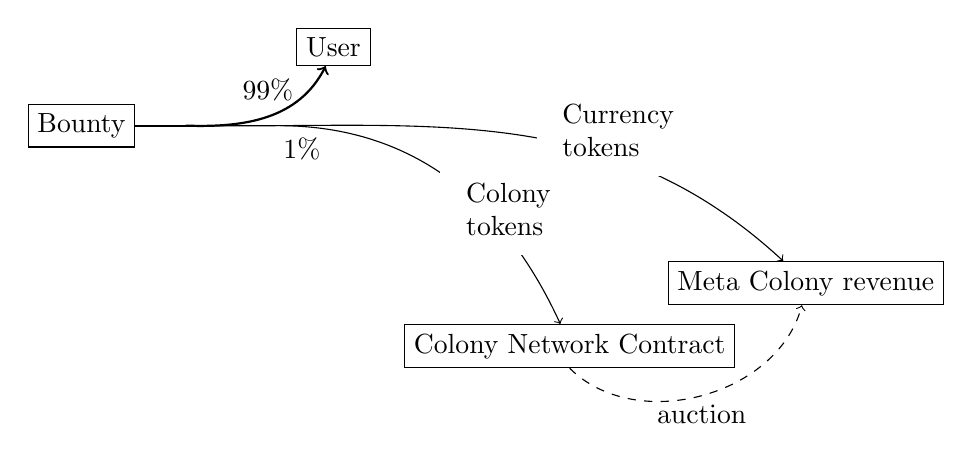
\begin{tikzpicture}
  \node at (-4,0) (dummy) {};
  \node[draw] at (-5.2,0) (bountybox) {Bounty};
  \node at (-2.8,0) (bounty) {}
   (bountybox.east) edge[-, thick] (dummy.east)
   (dummy.east) edge[-] (bounty.east);
   \node at (-2.4,-0.3) {{1\%}};
  \node[draw] at (-2,1) (user) {User};
  \node[draw] at (1,-2.8) (cnc) {Colony Network Contract};
  \node[draw] at (4,-2) (root) {\rc\ revenue}
    (dummy.east) edge[->, bend right=40,out=-25,thick] node[above=2pt] {99{\%}} (user)
    (dummy.east) edge[->, bend left=30,out=12] node[fill=white,right=10pt] {\begin{tabular}{l} Currency \\ tokens\end{tabular}} (root)
    (bounty.east) edge[->, bend left=30,out=35] node[fill=white, below right=-5pt] {\begin{tabular}{l} Colony \\ tokens\end{tabular}} (cnc)
    (cnc.south) edge[->, bend right=60, dashed] node[below] {auction} (root)
    ;
 \end{tikzpicture}
 \caption{Summary of the revenue split upon payout for a task.}
 \label{fig:revenueSplit}

\end{figure}

The fees thus collected are sent to either the \rc\ (if the payment was in Ether or another whitelisted token) or the Colony Network Contract (if it was in a colony's token).

This idea of a fee is a little unusual for such a decentralised system. One of the appeals of decentralised systems on Ethereum is that other than gas costs, they do not seek rent and are free to use. However, the Network Fee is vital in ensuring the game theoretic security of the Colony Network's reputation mining and governance processes by providing underlying value to the CLNY held by Meta Colony members. Importantly, this fee is not payable to any centrally controlled entity, but rather to the Meta Colony. Anybody may contribute to the Meta Colony and claim a share of these fees proportional to their contribution. We believe that the benefit of being part of a secure, well supported network will ultimately be appealing enough that a small fee to pay for its existence will be acceptable.

The presence of this fee means we have to make some considerations which would otherwise be irrelevant. Primarily, we will need to make `piggyback' contracts as hard as possible to make that might e.g. be used to pay out a task reward when a task was completed, but without sending the fee.

\subsubsection{The token auction}
As the network fee may be denominated in any ERC20 token, there is a need for a mechanism to liquidate arbitrary bundles of tokens -- the token auction. The colony tokens collected are auctioned off by the Colony Network Contract, with the auctions denominated in \rcts, the proceeds of which are burnt. These auctions --- one for each type of token collected --- occur on a regular basis of once a month.

We believe such a mechanism will be beneficial for the \rcths\ (whose \rcts\ gain value by having an explicit use beyond reputation mining) and the \rc\ itself (by reducing the supply of \rcts\ and thus making any future minting more valuable). It also provides an immediate mechanism of price discovery for the colony tokens, which are unlikely to be traded on third-party exchanges until much later in the lifetime of the colony. By auctioning off the collected tokens, we also prevent the \rc\ collecting a large number of different tokens that it has to manage, which would prove cumbersome and annoying for the colony.




\newpage
\section{Allowing More Complex Behaviour}\label{sec:special-cases}


% \subsection{Example Configurations}\label{sec:example-configs}
The protocol described in this document is concerned with what happens on the Ethereum blockchain. Users of the network however are not expected to ever interact with the contracts manually; instead they will be using front-end applications that make the network's functionality easy to use.

In any colony application we expect a certain amount of \textbf{front-end abstraction} in which complex tools and concepts are presented for the users' convenience, and translated in the background into a sequence of contract interactions on the colony network.

Front-end abstraction lets us realise certain functionality that doesn't \emph{seem} to be part of our protocol by combining the simple elements we have designed in inventive ways. The remainder of this section describes some such cases.

\subsection{Salaried positions}\label{sec:salary}

The work-for-payment model in the colony network is based around tasks, and on the surface this implies colony-worker relationships that are purely transactional. However the system is flexible enough to accommodate a wider range of employment models. One such example is a \emph{salaried position}.

A salaried position could be realised by creating a special domain representing the position to be filled. The domain could be issued the salary through a priority funding proposal. The employee would be the only person with reputation within that domain and would be able to withdraw funds by creating and self-assigning placeholder tasks that are funded from the domain's funding pot. A good user interface could hide these implementation details from the users and render salaried positions differently from regular domains.

\subsection{Awarding reputation for work not captured by tasks}

All reputation decays over time, as described in Section \ref{sec:reputation}. This prevents an eternal `reputation aristocracy' and allows reputation to be meaningful even after major changes in the colony token's value.

Reputation is awarded when a user receives payment of colony tokens --- most commonly as payout from a task, but sometimes from dispute resolution and, in the case of the \rc, from the reputation mining process. We can use the task payout mechanism to award users extra reputation provided there is consensus to do so.

Consider the scenario in which a founder, or an important early contributor to a colony has almost no reputation left by the time the colony starts earning revenue; perhaps the development of the product took a long time or perhaps the reputation decay rate was sub-optimally high for the particular colony.\footnote{Finding an optimal decay rate for reputation in the network will depend on empirical data collected from early colonies.} Or perhaps the founder was doing a lot of intangible work to get the colony off the ground in the first place and so was never compensated properly through the task system. To get around the limitations of the reputation system and to re-integrate the founder (and make them eligible to receive their rewards), the colony can create a special task that is solely designed to award reputation they are due. To qualify for the payout of tokens (and thereby the reputation), the user in question would have to give the same number of tokens back to the colony. Again, a good frontend abstraction could make such reputation awards easy and intuitive.

The important point is that any limitations imposed by the system can be weakened if there is consensus to do so. The system should not stand in the way of consensus, it should just provide conflict resolution mechanisms for those times in which there is dissent.

\subsection{Objections by non-members}

Having reputation is a prerequisite for creating an objection and triggering the dispute process. Therefore, if an outsider is hired by a colony to perform a task, they will not, on their own, be able to object to the evaluation of their work. However, a good colony frontend may allow them to create the template for an objection, effectively calling for members of the colony to support it and submit the objection to the colony network on-chain on their behalf.

This is analogous to a member staking only 10\% of the required amount and waiting for further support from their peers (Section \ref{sec:costs-of-disputes}), with the difference being that without any third party support, this `objection' would never be processed on-chain.

\subsection{Proposing an arbitrary transaction by the \ascode{Colony} contract}\label{sec:arbitrary-transaction}
Of course, it is possible that a colony will want to engage in some behaviour that we haven't foreseen, that could be implemented in a contract outside the control of the Colony Network. To that end, we wish to have a mechanism by which a colony can create an arbitrary transaction on the blockchain to interact with contracts and tokens without requiring the network to explicitly support them. As they are powerful, such transactions should be rare occurrences requiring high support thresholds.

Formally, proposing that a colony make an arbitrary transaction on the blockchain is no different from an objection; however the proposal is to change the value of a special variable from zero to the value of the transaction data of the proposed transaction. Such a proposal requires the entire colony to be able to vote (both token holders and reputation holders), as it concerns actions taken `by the contract as a whole'. In the event the proposal is successful, the special variable is set. Another subsequent transaction --- able to be made by anyone --- is able to call a function that executes the transaction in the special variable, and resets it to zero if successful.

\newpage
\section{Conclusion}\label{sec:conclusion}

We have described and defined the Colony Protocol --- an organisational operating system built on Ethereum. It provides a general purpose framework for the creation, management, and operation of decentralised organisations of various kinds.

The specification contained herein represents our current best description of the Colony Protocol. It is however, a working document, and it should be expected that the final specification will differ substantively, both as a consequence of the rapidly changing technological landscape, and the refinement of our understanding of the requirements of decentralised organisation through iterative cycles of development and user testing.

\subsection*{Acknowledgments}

% If you are submitting a PR, feel free to add your name, in alphabetical order by surname.

The authors would like to thank the following people for their comments, suggestions, and other contributions: Alexei Akhounov, Alex Amsel, Sebastian Klier, and Daniel Kronovet.

\bibliographystyle{./src/bibliography/custom.bst}
\bibliography{./src/bibliography/biblio}

\appendix
\newpage
% \clearpage
\section{Gas-Efficient Reputation Penalty in Dispute Resolution}\label{appendix:rep-transfer}

Once a dispute has been raised and settled one way or the other, the users on the losing side will lose reputation and those on the winning side will gain it. If there is then a disagreement during the reputation mining mechanism, we must be able to calculate on-chain, in a gas-efficient way, a specific reputational consequence of the dispute being settled. A dispute may affect the reputations of many users, but all of these reputation changes are represented by only a single entry in the `reputation update log', so it is necessary to expand upon the process used to resolve this.

Given that users are able stake small amounts on each objection, an arbitrarily large number of users could theoretically be involved. Gas limits dictate that we must therefore not have any (on-chain) loops in this implementation.

\subsection{Staking}

As noted in Section \ref{sec:costs-of-disputes}, an objection requires 0.1\% of the reputation queried and 0.1\% of the corresponding fraction of tokens to be staked' to be considered valid, but that just 10\% of this amount is sufficient in order to create such a proposal. The exact numerical values of how much reputation and how many tokens are needed, is set at the time the proposal is first created. We proceed with a detailed example.

Let us consider a situation where an objection requires 600 tokens and 1200 reputation points to activate. User A initiates the objections and puts up a stake of 100 tokens. In order to do this, A must have at least 200 relevant reputation points at the time. Assume that users B and C support the objection, staking 200 and 300 tokens (and having 400 and 600 reputation points) respectively.

\begin{table}[ht]
\centering
\caption{A table of stakes showing part of what is recorded during the dispute process up to the point where the `change' side has received enough support of 600 total tokens staked.}
\begin{tabular}{|c|c|c|c|c|}
\hline
\textbf{Stake \#} & \textbf{User}  & \textbf{Staked Tokens} & \textbf{$\Sigma^+$} \\ \hline
1 & A & 100           & 100                                                                                          \\ \hline
2 & B & 200           & 300                                                                                           \\ \hline
3 & C & 300           & 600                                                                                           \\ \hline
\end{tabular}
\end{table}
For simplicity, the table does not contain entries for reputation. The corresponding amounts of reputation at risk are implied.

Once the cumulative backing ($\Sigma^+$) reaches the threshold required (600) the objection becomes active. Now we assume that two users (D and E) oppose the objection with matching funds of 150 and 450 respectively.\footnote{We write negative numbers in the table to denote \emph{opposing} stake.} Once the cumulative backing on the keep side ($\Sigma^-$) reaches the required threshold (-600) a dispute is triggered.

\begin{table}[ht]
\centering
\caption{A table of stakes showing part of what is recorded during the dispute process up to the point where both the `change' and `keep' sides have received 600 tokens of support.}
\begin{tabular}{|c|c|c|c|c|c|}
\hline
Stake \# & User  & Staked Amount & $\Sigma^+$ & $\Sigma^-$ \\ \hline
1 & A & 100           & 100                      & 0                                                                       \\ \hline
2 & B & 200           & 300                      & 0                                                                       \\ \hline
3 & C & 300           & 600                      & 0                                                                       \\ \hline
4 & D & -150          & 600                      & -150                                                                    \\ \hline
5 & E & -450          & 600                      & -600                                                                    \\ \hline
\end{tabular}
\end{table}

We assume that, in the dispute, the initiating users (A, B and C) were found to have been wrong and so will lose some of their stake. To keep this example simple, let us pretend that they lose 50\% of their staked tokens to the opposing side (D and E). They will also lose a corresponding amount of relevant reputation, or all of their relevant reputation, whichever is smaller.

We will assume that all users have the appropriate amount reputation to lose (i.e. A, B and C did not lose their reputation between the time of backing this proposal and the resolution of the dispute). We will also assume the dispute only affected domain reputation, not skill reputation.\footnote{In the case of affecting both, the number of updates required is doubled.} There are four transfers of reputation that must occur here:

\begin{enumerate}
\item User A loses 100 reputation to User D
\item User B loses 50 reputation to User D
\item User B loses 150 reputation to User E
\item User C loses 300 reputation to User E
\end{enumerate}

Indeed, in a group of $m$ people where some owe the others a debt, the maximum number of transfers required to make everyone whole is equal to $m-1$. If the reputation being lost has $p$ parents and $c$ children, there are up to $p+c+1$ domain-totals to be updated (as some reputation is destroyed), $p+c+1$ reputations for the losing user, and $p+1$ totals for the gaining user (who does not receive any reputation in any child domains). Thus there are up to $3+3p+2c$ reputation updates that must occur at each of these steps. There are therefore $(m-1)\times(3+3p+2c)$ reputation updates in total. In the event of a disagreement regarding the reputation state, we must be able to access the $n^{th}$ update directly when calculating an update on-chain. This is made possible by additional logging of data when stakes are made.

When a user stakes and opposes some existing stake that does not yet have a counterpart, we record the stakes that it is matching against as well as any remainder.

\begin{table}[ht]
\centering
\caption{Table showing additional data recorded for stakes that match against earlier stakes on the opposite side.}
\begin{tabular}{|c|c|c|c|c|c|}
\hline
Stake & Match From & Match To & Remainder & Tx \# From & Tx \# To\\ \hline
-150  & 1          & 2        & 50      & 1 & 2 \\ \hline
-450  & 2          & 3        & 0       &  3 & 4 \\ \hline
\end{tabular}
\end{table}

When staking, the user supplies the `Match From' and `Match To' arguments. These can be checked to be correct on-chain in constant gas by using the values of $\Sigma^+$ and $\Sigma^-$ recorded alongside previous stakes, and the remainder from the previous match. Then, when a miner is asked to prove a particular transaction has been included, they can point to the row in this log that contains that transaction without the contract having to iterate over an arbitrarily long list. The user's client is required to do this iteration locally to find the row, but this does not require any gas expenditure.

\subsection{Exact matching}\label{sec:exactMatching}

For the `reputation update log' to work correctly, we must know exactly how many reputation updates we have to consider. In the above example, it was $4\times(3+3p+2c)$, which could be calculated and recorded easily in the update log. However, consider an example where the staked amounts were

\begin{table}[ht]
\centering
\caption{An example staking for each side where fewer than the upper limit of transfers for four people are required. Only two transfers are required to exactly balance the users.}
\begin{tabular}{|c|c|c|c|c|c|}
\hline
Stake \# & User  & Staked Amount & $\Sigma^+$ & $\Sigma^-$ \\ \hline
1 & A & 100           & 100                      & 0                                                                       \\ \hline
2 & B & 200           & 300                      & 0                                                                       \\ \hline
3 & C & -100           & 300                      & -100                                                                       \\ \hline
4 & D & -200          & 300                      & -300                                                                    \\ \hline
\end{tabular}
\end{table}

Even though there are four people, only two transfers are required --- from user A to user C, and from user B to user D. This is because the users have accidentally matched themselves exactly, and so one transaction makes two users `whole'. In order to accommodate this possibility in the reputation update log, we insert dummy reputation transfers in the log whenever an exact match occurs:

\begin{table}[ht]
\centering
\caption{Table showing what is recorded for stakes that match against earlier stakes on the opposing side, in the case where some match exactly. The entries with 0 stake are used to ensure there are four transactions recorded, even if not all are needed.}
\label{tab:matchFromTo}
\begin{tabular}{|c|c|c|c|c|c|}
\hline
Stake & Match From & Match To & Remainder & Tx \# From & Tx \# To \\ \hline
-100  & 1          & 1        & 0   & 1 & 1     \\ \hline
 0 & 0          & 0        & 0      & 2 & 2   \\ \hline
-200 & 2          & 2        & 0    & 3 & 3    \\ \hline
 0 & 0          & 0        & 0      & 4 & 4   \\ \hline
\end{tabular}
\end{table}

These dummy insertions occur whenever the remainder is 0 --- i.e. when the new stake has exactly matched the first unmatched stakes. This ensures that this log always describes as many transactions as there are people (the last entry is always a dummy transaction as the final transaction will always make two users whole). This means that regardless of how the users have matched up against each other, the event that is recorded in the reputation update log will have a known number of transactions equal to the number of staking users, even if some of those are `null' transactions.

% \subsection{Generalisation}
%
% This procedure can also be extended to account for stakes being made in arbitrary orders (i.e. not all of one side followed by all of the other). This can be achieved by making the indices in the `Match From' and `Match To' columns only refer to stakes on one side or the other, and keeping matching lists that map those indices onto the stakes. Altering our first example slightly, we might end up with the stakes in table \ref{appa:modifiedexample} and the log entries in table \ref{appa:modifiedexamplelog}. The list of positive stakes would be [1, 3, 4] and the list of negative stakes would be [2, 5]. The `Match From' and `Match To' indices then refer to the list corresponding to the opposite sign of the stake currently being considered.
%
% \begin{table}[ht]
% \centering
% \caption{Generalised case of staking where stakes from each side occur in an arbitrary order.}
% \label{appa:modifiedexample}
% \begin{tabular}{|c|c|c|c|c|}
% \hline
% User  & Staked Amount & $\Sigma^+$ & $\Sigma^-$ \\ \hline
% A & 100           & 100                      & 0                                                                       \\ \hline
% B & -150           & 100                      & -150                                                                     \\ \hline
% C & 300           & 400                      & -150                                                                       \\ \hline
% D & 200          & 600                      & -150                                                                    \\ \hline
% E & -450          & 600                      & -600                                                                    \\ \hline
% \end{tabular}
% \end{table}
%
% \begin{table}[ht]
% \centering
% \caption{Equivalent of Table \ref{tab:matchFromTo} in the case where stakes can be made on either side in any order. The `Match From' and `Match To' indices now refer to lists of stakes for each side, which are recorded separately.}
% \label{appa:modifiedexamplelog}
% \begin{tabular}{|c|c|c|c|c|c|}
% \hline
% Stake & Match From & Match To & Remainder & Tx \# From & Tx \# To\\ \hline
% -150  & 1          & 1        & -50      & 1 & 1 \\ \hline
% 300   & 1          & 1        & 250      & 2 & 2 \\ \hline
% -450  & 2          & 3        & 0       &  3 & 4 \\ \hline
% 0  & 0         & 0        & 0 & 5 & 5            \\ \hline
% \end{tabular}
%
% \end{table}
%
% So for example, in Table \ref{appa:modifiedexamplelog}, the stake of -150 is matching against the stake at index 1 in the `positive stake' list which is stake number 1 i.e. the stake from user A. The stake of 300 is matching against the stake at index 1 in the `negative stake' list, which is stake number 2 i.e. the (remainder of the) stake from user B.

\newpage
\clearpage
\section{Reputation Decay Calculation Details}\label{appendix:rep-decay}

Reputation in any skill decays by a factor of two every \repdecayduration\ days. At each update (i.e. after every \miningcycleduration\ hours), the new decayed value ($u_{\rm new}$) is calculated by

$$u_{\rm new} = u_{\rm old} \times \exp\left(-\frac{\ln 2}{\decayfactor}\right) = u_{\rm old} \times \exp\left(-k\right).$$

This calculation is applied separately to each user's skill, as well as the number that represents the total of all of those skills in the colony. Due to rounding error with the integer representation on the blockchain, these numbers will drift away from each other. However, we can show the accumulated error will be negligible. The amount of reputation that will be incorrectly missing after the first iteration will be, on average. $0.5N$ reputation wei, where $N$ is the number of users that have this skill.\footnote{This ignores the incorrectly lost reputation from rounding error introduced when decaying the colony-wide sum of the relevant reputation, but as there is only one total and many more users, ignoring it does not change our conclusions. We also note that there is an implicit assumption here that all users have the same amount of reputation; this is a worst-case assumption, as if it is not true then once some users have lost all their reputation the reputation incorrectly lost on each cycle will drop below $0.5N$.} The 0.5 is the average fractional part lost during each calculation.

After the second iteration, the amount of reputation that is incorrectly missing is

$$0.5N\exp\left(-k\right) + 0.5N.$$


The second term here is the incorrectly lost reputation from this second set of calculations. The factor of $\exp\left(-k\right)$ has been introduced to the term representing the incorrectly lost reputation from the first set of calculations because some of that incorrectly lost reputation would have correctly decayed away by this point, and so it shouldn't be considered incorrectly lost.

It is apparent that this is a geometric series, and after $b$ cycles of reputation update have passed, the amount of reputation incorrectly missing ($R_{\rm m}$) is
$$R_{\rm m} = \frac{N}{2} \left(\frac{1-\exp\left(-bk\right)}{1-\exp\left(-k\right)}\right)$$

\noindent where we have used the standard result for the sum of a geometric series. If we started with $R_0$ reputation, then the ratio of the incorrectly missing reputation to the total the colony believes exists is

$$\frac{R_{\rm m}}{R_0\exp\left(-bk\right)}.$$


This ratio becomes 1 when
$$ b = \frac{1}{k}\ln\left(\frac{2R_{\rm 0}}{N}\left(1-\exp\left(-k\right)\right) +1   \right)$$


\noindent which, for conservative values of $R_0 = 200\times10^{18}$ and $N=1000000$ occurs after 38011 iterations, or over \timetofail\ years for a \miningcycleduration\ hour mining cycle. At this point, even though the colony believes some amount of reputation exists, no users have it, and no users can make decisions related to this type of reputation.

This is the end-of-life for an inactive colony; if no activity takes place in it for \timetofail\ years that is worthy of earning reputation, then the colony will be irrecoverable --- no-one will be able to create tasks to earn further reputation. This seems like a reasonable failure mode for an inactive colony, and it would take longer to reach for smaller colonies (with fewer rounding errors).

We now consider the case of an active colony. If the colony is active and creates $A$ new reputation at every update cycle, how does the ratio between the figure taken to be the total reputation and the incorrectly missing reputation change over time?

$R_{\rm m}$ remains the same in this situation, but the total reputation the colony believes exists increases by $A$ each cycle. After $b$ iterations, we can show that the total reputation the colony believes exists is

$$R_{\rm 0}\exp\left(-bk\right) + A\frac{1-\exp\left(-bk\right)}{1-\exp\left(-k\right)}.$$


As $b$ tends to infinity --- which represents the regime of a colony in a steady state --- the ratio between this and $R_{\rm m}$ tends to
$$\frac{N}{2A}$$

\noindent i.e. for the discrepancy to be small between what the colony thinks the total reputation inside it is and the sum of all users' reputations, the reputation earned in each cycle should, on average, be much larger than the number of users. Given that reputation will be expressed in terms of numbers on the order of $10^{18}$, this seems assured.

For calculating the exponential decay, we will use the first-order Taylor expansion of the exponential decay i.e. we approximate $\exp\left(-k\right)$ as $1-k$. Given that $k$ is small, this will be a good approximation --- the second order term is on the order of $10^{-7}$. This error will cause all reputations to decay slightly faster than an exponential, but otherwise will have no effect.

When calculating the decay, in order to accommodate the fact that we are multiplying by a value close to one and only integers are available in Solidity, we will multiply the user's reputation by $K(1-k)$ (calculated off-chain), for some large value of $K$, and then divide by the same large factor $K$.



\end{document}
